\documentclass[12pt,a4paper]{article}
\usepackage[top=3cm,bottom=3cm,left=2.5cm,right=2.5cm]{geometry}
\usepackage[utf8]{inputenc}
\usepackage[T1]{fontenc}
\usepackage{amsmath}
\usepackage{amsthm}
\usepackage{amsfonts}
\usepackage{amssymb}
%\usepackage{graphicx}
\usepackage{enumerate}
\usepackage{txfonts}
\usepackage[dvipsnames]{xcolor}
\usepackage{tcolorbox}
\usepackage{hyperref}
\hypersetup{
	colorlinks = true}
\usepackage{tikz}
\usetikzlibrary{calc}
\usetikzlibrary{cd}
\usepackage{tikz-3dplot}



% ================SET Color for the environment
\tcbuselibrary{theorems}
\tcbuselibrary{breakable}
\newtcbtheorem
	[number within=subsection]% init options
	{definition}% name
	{Definition}% title
	{%
		breakable,
		colback=Emerald!10,
		colframe=cyan!40!black,
		fonttitle=\bfseries,
	}% options
	{def}% prefix
	
\newtcbtheorem
	[use counter from =definition]% init options
	{theorem}% name
	{Theorem}% title
	{%
		breakable,
		colback=Salmon!20, 
		colframe=Salmon!90!Black,
		fonttitle=\bfseries,
	}% options
	{thm}% prefix
	
\newtcbtheorem
[use counter from =definition]% init options
{proposition}% name
{Proposition}% title
{%
	breakable,
	colback=OliveGreen!10,
	colframe=Green!70,
	fonttitle=\bfseries,
}% options
{prop}% prefix

\newtcbtheorem
[use counter from =definition]% init options
{example}% name
{Example}% title
{%
	breakable,
	colback=green!5,
	colframe=green!35!black,
	fonttitle=\bfseries,
}% options
{example}% prefix


\newtcbtheorem
[use counter from =definition]% init options
{lemma}% name
{Lemma}% title
{%
	breakable,
	colback=SeaGreen!10!CornflowerBlue!10,
	colframe=RoyalPurple!55!Aquamarine!100!
	fonttitle=\bfseries,
}% options
{lemma}% prefix


\newtcbtheorem
[use counter from =definition]% init options
{corollary}% name
{Corollary}% title
{%
	breakable,
	colback=JungleGreen!10!Cerulean!15,
	colframe=CornflowerBlue!60!Black,
	fonttitle=\bfseries,
}% options
{coro}% prefix



% ==================================


\author{Liu Zhizhou}
\title{Basic concepts with proofs in \emph{Dynamical Systems}, Topological Dynamics and Ergodic Theory}
\begin{document}
	\maketitle
	
	This is a lecture notes of the book \cite{brin2002introduction}, but full of details.
	
	\tableofcontents
	
	\newcommand{\N}{\mathbb{N}}
	\newcommand{\frakC}{\mathfrak{C}}
	
	
	
	
	\section{Topological Dynamics}
	\begin{definition}{Basic Definition in Topological Dynamics}{basic def}
		We introduce the definitions for dynamical systems, homemorphism, semiconjugacy/conjugacy, isometry.
		\begin{enumerate}
			\item A \emph{topological dynamical system} $(X,f)$ is a topological space $X$ and a continuous map $f:X\rightarrow X$. In the context, we always assume $X$ is compact and metric (with metric $d$) for simplicity.
			\item A continuous map $f$ is called \emph{homemorphism} if it is bijective and the inverse is continuous.
			\item Let $f:X\rightarrow X$ and $g:Y\rightarrow Y$ be  topological systems. A \emph{topological semiconjugacy} from $g$ to $f$ is a surjective continuous map $\pi:Y\rightarrow X$ such that $f\circ \pi = \pi \circ g$. Then $(X,f)$ is a \emph{factor} of $(Y,g)$ and $(Y,g)$ is an \emph{extension} of $(X,f)$. If $\pi$ is homemorphism, then it is called a \emph{topological conjugacy}. 	
			\begin{tikzcd}
				&Y \arrow[r, swap, "g"] \arrow[d, "\pi"] &Y \arrow[d, swap, "\pi"] \\
				&X \arrow[r, "f"]  &X
			\end{tikzcd}
			\item If $(X,d)$ and $(Y,d')$ are metric spaces, then $f:X\rightarrow Y$ is an \emph{isometry} if $d'(f(x_1),f(x_2))=d(x_1,x_2)$, for all $x_1,x_2\in X$. (The same definition in normed space)
		\end{enumerate}
	\end{definition}
	Be careful that $f^n(x)$ always represents $f\circ\dots\circ f$ for $n$ times, or in terminology, we say that $f$ iterates $n$ times.
	
	\subsection{Properties of Limit Sets}
	\begin{definition}{$\omega$ and $\alpha$ limit points and sets}{}
		Here we give a definition for $\omega$ and $\alpha$ limit points and sets. Let $f:X\rightarrow X$ be a topological dynamical system. Let $x\in X$. 
		\begin{enumerate}
			\item A point $y\in Y$ is an $\omega$ limit point of $x$ if there is a sequence of natural numbers $n_k\to \infty$ (as $k\to \infty$) such that $f^{n_k}(x)\to y$.
			\item The $\omega$ limit set of $x$ is the set $\omega(x)$ or denoted $\omega_f(x)$ of all $\omega$ limit points of $x$.
			\item If $f$ is invertible, the $\alpha$ limit point and set of $x$ is just change $f^{n_k}$ from the above definition to $f^{-n_k}$. In other words, the $\alpha$ limit sets of $x$ for $f$ is the $\omega$ limit sets of $x$ for $f^{-1}$. 
		\end{enumerate}
	\end{definition}
	Note that the limit sets we defined here is just like the limit sets in sequence of numbers.
	\begin{proposition}{Equivalent definition}{}
		 Let $f:X\rightarrow X$ be a topological dynamical system. Let $x\in X$. Then
		 $$
		 \omega(x)=\bigcap_{n\in\N}\overline{\bigcup_{i\geq n} f^i(x)}.
		 $$
		 Consequently, if $f$ is invertible, then
		 $$
		 \alpha(x)=\bigcap_{n\in\N}\overline{\bigcup_{i\geq n} f^{-i}(x)}.
		 $$
	\end{proposition}
	\begin{proof}
		We need to prove two sides of inclusion. Firstly, assume $y\in\omega(x)$, then exists $\{n_{k}\}$ infinite sequence with $n_k\to \infty $ such that $f^{n_k}(x)\to y$. Our aim is to prove $y\in \bigcap_{n\in\N}\overline{\bigcup_{i\geq n} f^i(x)}$, i.e for all $n\in\N$, $y\in \overline{\bigcup_{i\geq n} f^i(x)}$. 
		
		To show this, note that $y\in \overline{A}$ for some set $A$ if and only if for any $\epsilon>0,$ there exist $z\in A$ such that $d(y,z)<\epsilon$, i.e. $A\cap B(y,\epsilon)\neq \emptyset$ for any $\epsilon>0$.
		
		Now for any $\epsilon>0$, since $f^{n_k}(x)\to y$, we have for any $n\in \N$, there exist $n_k\geq n$ such that $f^{n_k}(x)\in B(y,\epsilon)$. Thus, $\forall n\in \N,$ we have
		$\bigcup_{i\geq n} f^i(x)\cap B(y,\epsilon)\neq \emptyset,$
		which means $y\in \overline{\bigcup_{i\geq n} f^i(x)}$ for all $n\in \N$. 
		
		Conversely, assume $y\in\bigcap_{n\in\N}\overline{\bigcup_{i\geq n} f^i(x)}.$ Then $y\in \overline{\bigcup_{i\geq n} f^i(x)}$ for all $n\in \N$. So that $\forall n\in \N,$ we have
		$\bigcup_{i\geq n} f^i(x)\cap B(y,\epsilon)\neq \emptyset.$ Hence there must exist $\{n_k\}$ with $n_k\to \infty$ such that $f^{n_k}(x)\to y$.
	\end{proof}
	The observation we used in the proof of the proposition is used to express the feeling of points being approximated by sequence in the topological space. And this proposition makes the connection between 'limit' in the sense of sequence and the 'limit' in the sense of closed sets. This proposition is somewhat trivial because we have similar results for limit points in sequence of numbers.

	
	
	
	\begin{proposition}{closed and $f$ invariant of limit sets}{}
		Both $\omega$ and $\alpha$ limit sets are closed and $f$ invariant.
	\end{proposition}
	\begin{proof}
		By the equivalent definition of $\omega$ and $\alpha$ limit sets, since it is the intersection of closed sets, it is automatically closed. For the invariant property, choose $y\in \omega(x)$, then exists $\{n_k\}$ such that $f^{n_k}(x)\to y$. Consider $f(y)$. Since $f$ is continuous, we should have $f^{n_k+1}(x)\to f(y)$, which shows $f(y)\in \omega(x)$. Here the sequence is $n_k+1$.
		
		For $\alpha$ limit sets, choose $y\in \alpha(x)$, then exists $\{n_k\}$ such that $f^{-n_k}(x)\to y$. Consider $f(y)$ also. Since $f$ is continuous, we should have $f^{-n_k+1}(x)\to f(y)$, which shows $f(y)\in\alpha(x)$. Here the sequence is $n_k-1$. 
	\end{proof}


	\subsection{Recurrent and Non-wandering Sets}
	\begin{definition}{Recurrent and Non-wandering Points and Sets}{}
		Let $f:X\rightarrow X$ be a topological dynamical system. Let $x\in X$. 
		\begin{enumerate}
			\item A point $x$ is called \emph{(positively) recurrent} if $x\in \omega(x)$;
			\item The set $R(f)$ is defined to be the set that consists of all recurrent points;
			\item A point $x$ is \emph{non-wandering} if for any neighborhood $U$ of $x$, there exists $n\in \N$ such that $f^n(U)\cap U\neq \emptyset$;
			\item The set $NW(f)$ is defined to be the set that consists of all non-wandering points.
		\end{enumerate}
	\end{definition}
	What does $f(U)\cap U$ mean? Take $x\in f(U)\cap U$, then $x\in U$ belongs to the image of $U$. That is, the image of a point in $U$ after 1 iteration. Generally, the $f^n(U)\cap U$ is the set of points after $n$ iterations beginning with a point in $U$. Likewise, what does $f^{-n}(U)\cap U$ mean? It means the set of points that will lie in $U$ after $n$ iterations. 





	\begin{proposition}{}{}
		We have the following properties:
		\begin{enumerate}
			\item The set $R(f)$ is $f$ invariant;
			\item The set $NW(f)$ is closed and $f$ invariant;
			\item $NW(f)$ contains $\omega(x)$ and $\alpha(x)$ for all $x\in X$.
		\end{enumerate}
	\end{proposition}
	\begin{proof}
		To show the first property, we need to show that if $x$ is a recurrent point, i.e. $x\in \omega(x)$, then $f(x)\in \omega(f(x))$. If there exists $\{n_k\}$ with $n_k\to\infty$ such that $f^{n_k}(x)\to x$, then the same sequence ensures $f^{n_k}(f(x))=f(f^{n_k}(x))\to f(x)$, since $f$ is continuous.
		
		To prove $NW(f)$ is closed, choose $\{x_n\}$ with $x_n\to x$ where $x_n\in NW(f)$. For any neighborhood $U$ contains $x$, there exists $r$ such that $B(x,r)\subset U$. And for any $\epsilon>0$, there exists $N$ such that $x_N\in B(x,\epsilon)$. Then there must exists $x_N\in B(x,r)\subset U$. Since $x_N$ is non-wandering, there exists $n\in \N$ such that $f^n(U)\cap U\neq \emptyset$.
		
		And $NW(f)$ is $f$ invariant because if $x\in NW(f)$, then there exists $n$ such that $f^n(U)\cap U\neq \emptyset$, i.e. there exists $y\in U$ such that $f^n(y)\in U$. Consider $f(x)$, for any neighborhood $U$ of $f(x)$, then $f^{-1}(U)$ will also be open neighborhood of $x$. Thus there exists $n$ and $y\in f^{-1}(U)$ such that $f^n(y)\in f^{-1}(U)$. So $f^{n}(f(y))$ will be in $U$ and $f(y)\in U$, which shows $f^n(U)\cap U\neq \emptyset$. 
		
		Finally, for any fixed $x$, assume $y\in \omega(x)$, there must exists $\{n_k\}$ with $n_k\to\infty$ such that $f^{n_k}(x)\in B(y,\epsilon)$ for any $\epsilon>0$. Then $f^{n_2-n_1}\circ f^{n_1}(x)=f^{n_2}(x)\in B(y,\epsilon)$. This shows that for any neighborhood $U$ contains $y$ there exists $N$ such that $f^N(U)\cap U\neq \emptyset$.
		
		For $y\in \alpha(x)$, the proof is similar. Just note that $f^{n_2-n_1}\circ f^{-n_2}(x)=f^{-n_1}(x)\in B(y,\epsilon)$.
	\end{proof}
	
	From the properties and the proof above, we can think of recurrence points as points, say $x$ that will have a subsequence of $f^{n}(x)$ that converges to itself. And non-wandering points are worse. It only grantees that for there exists sequence of points, say $y_k$, in neighborhood of $x$ such that  $f^{n_k} (y_k) \to x$ for some $n_k\to \infty$. From this, the fact that $R(f)\subset NW(f)$ is obvious. And it is also obvious that all periodic points (i.e. exists $N\in \N$ such that $f^N(x)=x$) and all stationary points (i.e. $f(x)=x$) are in $R(f)\subset NW(f)$.
	
	
	In fact, we have the following proposition.
	\begin{proposition}{}{}
		$\overline{R(f)}\subset NW(f)$.
	\end{proposition}
	
	
	
	
	\subsection{Topological Entropy}
	Topological entropy is the exponential growth rate of the number of essentially different orbit segments of length $n$. It measures the complexity of the orbit structure of a dynamical system. And we shall show that it is a topological invariant under conjugacy.
	
	We now define a metric $d_n(x,y)$ to measure the maximum distance between $x$ and $y$ after iterates for $n$ times. It is defined to be 
	$$
	d_n(x,y) =\max_{0\leq \leq n-1} d(f^k(x),f^k(y)).
	$$
	It is easy to see that $d_n\geq d_{n-1}$ and $d_1=d$. Moreover, we have the following proposition.
	\begin{proposition}{}{}
		Let $(X,d)$ be a compact metric space. Show that the metrics $d_i$ all induce the same topology on $X$.
	\end{proposition}
	\begin{proof}
		Let $B^n(x,r)=\{y\in X: d_n(x,y)<r\}$. To show $d_n$ and $d$ induce the same topology, it is equivalent to show that: (i) for any $\epsilon>0$, there exists $\delta>0$ such that $B^1(x,\delta)\subset B^n(x,\epsilon)$; and (ii) for any $\epsilon'>0$, there exists $\delta'>0$ such that $B^n(x,\delta')\subset B^1(x,\epsilon')$.
		
		For (i), choose $\delta= \epsilon$. Then for $y\in B^n (x,\delta)$, we have $d_n(x,y)\geq d(x,y)$ and $d_n(x,y)<\delta=\epsilon$, so $d(x,y)<\epsilon$, i.e. $y\in B^1(x,\epsilon)$.
		
		For (ii), since $f$ is continuous, $f^n$ must also be continuous. For the $\epsilon'>0$, there exists $\delta_n>0$ such that once $d(x,y)<\delta_n$, then $d(f^n(x),f^n(y))<\epsilon$. Let $\delta'=\min_n \delta_n$. Then for $y\in B^1(x,\delta')$, then we must have $y\in B^n (x,\epsilon')$, since we have $d_n(x,y)=d(f^n(x),f^n(y))<\epsilon'$ for all $n$. Therefore, $B^1(x,\delta')\subset B^n (x,\epsilon')$.
	\end{proof}
	
	\newcommand{\spn}{\text{span}}
	\newcommand{\sep}{\text{sep}}
	\newcommand{\cov}{\text{cov}}
	
	We then define three numbers respectively.
	\begin{definition}{spanning number, separated number, covering number}{}
		Fix $\epsilon>0$.
		\begin{enumerate}
			\item A subset $A\subset X$ is \emph{$(n,\epsilon)$ spanning} if for every $x\in X$ there is $y\in A$ such that $d_n(x,y)<\epsilon$. We denote the minimum cardinality of $A$ by $\spn(n,\epsilon,f)$; 
			\item A subset $A\subset X$ is \emph{$(n,\epsilon)$ separated} if any two distinct points in $A$ are at least $\epsilon$ apart in the metric $d_n$. Any $(n,\epsilon)$ separated set is finite. Let $\sep(n,\epsilon,f)$ denote the maximum cardinality of $A$.
			\item Let $\cov(n,\epsilon,f)$ be the minimum cardinality of a covering of $X$ by sets of $d_n-$ diameter less than $\epsilon$.
		\end{enumerate}
	\end{definition}
	 By compactness, there are finite $(n,\epsilon)$ spanning sets and covering sets, so that the corresponding numbers are finite. The separated number is also finite, since otherwise, by compactness, there is a convergent subsequence of the separated sequence $\{x_n\}$, this contradicts with $d(x_i,x_j)\geq \epsilon$. 
	 
	 Remember that $d_n(x,y)$ is the maximum distance after $n$ times iterations. Therefore, for instance, $\cov(n,\epsilon,f)$ measures the complexity after $n$ iterations. For fixed $\epsilon$, the more chaotic the map $f$ is, the smaller the covering number is. 
	 
	 In other words, think of $f^n(x)$ as continuous time model, i.e. $f^t(x),t\in \mathbb{R}_+$. Then for any fixed point $x$, $f^t(x)$ is like a 'noodle' with length $t$. Then, for any element $x$ in the spanning set $A$, there is noodle of radius $\epsilon$. And the spanning number is finite means that finite many noodles can span the compact space $X$. Also, separate number conuts the noodles in a different way. Instead of counting the minimum number that generates the whole space $X$, it counts for the maximum number of distinguishable noodles. And the only difference between spanning and covering is that in spanning, the noodles must be in shape of cylinder with radius (of every slice) less than $\epsilon$, while in covering, the noodles can be of arbitrary shape with diameter (of every slice) less than $\epsilon$.
	 
%	 \tdplotsetmaincoords{60}{80}
%	 \begin{tikzpicture}[scale=2,tdplot_main_coords]
%	 	\coordinate (O) at (0,0,0);
%	 	\tdplotsetcoord{P}{1}{70}{70}
%	 	\draw[thick,->] (0,0,0) -- (1,0,0) node[anchor=north east]{$x$};
%	 	\draw[thick,->] (0,0,0) -- (0,1,0) node[anchor=north west]{$t$};
%	 	\draw[thick,->] (0,0,0) -- (0,0,1) node[anchor=south]{$y$};
%	 	%\draw[-stealth,color=red] (O) -- (P);
%	 	\draw[dashed, color=red] (O) -- (Px);
%	 	\draw[dashed, color=red] (O) -- (Py);
%	 	\draw[dashed, color=red] (O) -- (Pz);
%	 	\draw[dashed, color=red] (Px) -- (Pxy);
%	 	\draw[dashed, color=red] (Py) -- (Pxy);
%	 	\draw[dashed, color=red] (Px) -- (Pxz);
%	 	\draw[dashed, color=red] (Pz) -- (Pxz);
%	 	\draw[dashed, color=red] (Py) -- (Pyz);
%	 	\draw[dashed, color=red] (Pz) -- (Pyz);
%	 	\draw[dashed, color=red] (Pxy) -- (P);
%	 	\draw[dashed, color=red] (Pxz) -- (P);
%	 	\draw[dashed, color=red] (Pyz) -- (P);
%	 \end{tikzpicture}
	 
	 
	 
	 
	 
	 
	 
	 
	 Intuitively, since circles are of diameter $2\epsilon$, we must have $\cov(n,2\epsilon,f)\leq \spn(n,\epsilon,f).$ And also, the $\epsilon$-separated noodles is enough to generate the space, so $\spn(n,\epsilon,f)\leq \sep(n,\epsilon,f)$. Rigorous proof and more information are presented in the following proposition.
	 \begin{proposition}{}{ineq cov}
	 	$\cov(n,2\epsilon,f)\leq \spn(n,\epsilon,f)\leq \sep(n,\epsilon,f)\leq \cov(n,\epsilon,f)$.
	 \end{proposition}
	\begin{proof}
		Suppose $A$ is an $(n,\epsilon)$ spanning set of minimum cardinality. Then the open balls of radius $\epsilon$ centered at the points of $A$ cover $X$. By compactness, there exists $\epsilon_1<\epsilon$ such that the balls of radius $\epsilon_1$ centered at the points of $A$ also cover $X$. Their diameter is $2\epsilon_1<2\epsilon$. Here we choose $\epsilon_1$ this way because the definition of covering sets needs sets of $d_n-$diameter less than $\epsilon$. Hence, we have the same number of covering set as the spanning set but this covering set might not be the minimum. Thus $\cov(n,2\epsilon,f)\leq \spn(n,\epsilon,f)$.
		
		Suppose $B$ is an $(n,\epsilon)$ separated set of maximum cardinality. Then for any $x\in X$, $d(x,y)\leq \epsilon$ for some $y\in B$, i.e. $\bigcup_{y\in B} B(y,\epsilon)$ spans $X$. However, this spanning set may not be the minimum, and thus $\spn(n,\epsilon,f)\leq \sep(n,\epsilon,f)$.
		
		Finally, suppose $\frakC$ is an $(n,\epsilon)$ covering set of maximum cardinality. If $\sep(n,\epsilon,f)< \cov(n,\epsilon,f)$, then there exists $\sep(n,\epsilon,f)$ $\epsilon$-separated points. However, note that at least a pair of separated points will lay in the same covering set by Pigeonhole Principle. This will leads to a contradiction since this pair of separated points will have distance strictly less than $\epsilon$.
	\end{proof}
	Note that $A,B$ consists of points but $CC$ is the collection of sets in the above proof.
	
	The entropy is defined as following. First, let
	$$
	h_\epsilon (f) = \limsup_{n\to \infty}\frac{1}{n} \log (\cov(n,\epsilon,f)).
	$$
	We have the following lemma.
	\begin{lemma}{}{}
		The limit $\lim_{n\to\infty}\frac{1}{n}\log(\cov(n,\epsilon,f))=h_{\epsilon}(f)$ exists and is finite. \label{lemma: limitexists}
	\end{lemma}
	\begin{proof}
		Let $U$ have $d_m$-diameter less than $\epsilon$, i.e. $\forall x,y\in U$, $\max_{i=0,\dots,m-1}d(f^i(x),f^i(y))<\epsilon$. Let $V$ have $d_n-$diameter less than $\epsilon$, i.e. $\forall x,y\in V$, $\max_{i=0,\dots,n-1}d(f^i(x),f^i(y))<\epsilon$. Then $\forall x,y\in U\cap f^{-m}(V)$, we have $x,y\in U$ and $f^m(x), f^m(y)\in V$, so that $U\cap f^{-m}(V)$ has $d_{m+n}$-diameter less than $\epsilon$. Hence 
		$$
		\cov(m+n,\epsilon,f)\leq \cov(m,\epsilon,f)\cdot \cov(n,\epsilon,f)
		$$
		since the number of $U\cap f^{-m}(V)$ kind set is $\cov(m,\epsilon,f)\cdot \cov(n,\epsilon,f)$ and the union must covers $X$ (for any $x\in X$ we can find a pair of $U,V$ such that $x\in U$ and $f^m(x)\in V$ by the definition of covering set). Now let $a_n=\log(\cov(n,\epsilon,f))\geq 0$ is sub-additive. Recall we have a lemma
		\footnote{Statement of the lemma: Let $\{a_n\}$ be a sub-additive sequence of non-negative real numbers, i.e. $0\leq a_{m+n}\leq a_m+a_n$ for all $m,n\geq 0$. Then $\lim_{n\to\infty} a_n/n = \inf_{n\geq 0} a_n/n$. And the proof of this lemma is first fix $n$ and consider $m=kn+r$, then using $\epsilon-N$ language to conclude.}
		 in sequence of numbers says that if $\{a_n\}$ is sub-additive and non-negative then
		$$
		\lim_{n\to\infty}\frac{a_n}{n}=\inf_{n\geq 0}\frac{a_n}{n}.
		$$
		Therefore in our situation, 
		$$
		\lim_{n\to\infty} \frac{1}{n} \log(\cov(n,\epsilon,f)) = \inf_{n\geq0}\frac{1}{n} \log(\cov(n,\epsilon,f)),
		$$
		also note that $1/n \log(\cov(n,\epsilon,f))$ is bounded from below (one of the lower bound is 0, obviously), we have the limit exists and is finite.
	\end{proof}
	Hence, we have 
	$$
	h_\epsilon(f) = \lim_{n\to\infty}\frac{1}{n}\log(\cov(n,\epsilon,f)).
	$$
	

	
	Since $\cov(n,\epsilon,f)$ increases monotonically as $\epsilon$ decreases (we need more noodles to cover the space if the diameter became thinner), $h_\epsilon (f)$ does as well. Thus, the limit
	$$
	h_{\text{top}}=h(f)=\lim_{\epsilon\to 0^+} h_{\epsilon}(f)
	$$
	exists (in the sense of $\mathbb{R}\cup \infty$). And we define it to be the topological entropy as below.
	\begin{definition}{topological entropy}{}
		Let $(X,d)$ be a compact metric space, and $f:X\rightarrow X$ a continuous map, the \emph{topological entropy} of $f$, denoted by $h_{\text{top}}(f)$ or simply $h(f)$, is defined as
		$$
		h_{\text{top}}(f) =h(f)=\lim_{\epsilon\to 0^+}h_{\epsilon}(f)=\lim_{\epsilon\to 0^+}\lim_{n\to \infty}\frac{1}{n}\log(\cov(n,\epsilon,f)).
		$$
	\end{definition}
	
	By previous inequality (Proposition \ref{prop:ineq cov}), we have
	$$
	\frac{1}{n}\log(\cov(n,2\epsilon,f))\leq \frac{1}{n}\log(\spn(n,\epsilon,f))\leq \frac{1}{n}\log(\sep(n,\epsilon,f))\leq\frac{1}{n}\log(\cov(n,\epsilon,f))
	$$
	and take $\limsup_{n\to \infty}$ or $\liminf_{n\to\infty}$ then take $\lim_{\epsilon\to 0^+}$, we will find
	\begin{align}
		h(f)&=\lim_{\epsilon\to 0^+} \limsup_{n\to\infty}\frac{1}{n}\log( \cov (n,\epsilon,f))=\lim_{\epsilon\to 0^+} \liminf_{n\to\infty}\frac{1}{n}\log( \cov (n,\epsilon,f)) \label{eq:hf=cov}\\   
		&=\lim_{\epsilon\to 0^+} \limsup_{n\to\infty}\frac{1}{n}\log(\spn(n,\epsilon,f))=\lim_{\epsilon\to 0^+} \liminf_{n\to\infty}\frac{1}{n}\log( \spn (n,\epsilon,f)) \label{eq:hf=spn}\\ 
		&=\lim_{\epsilon\to 0^+} \limsup_{n\to\infty}\frac{1}{n}\log(\sep(n,\epsilon,f))=\lim_{\epsilon\to 0^+} \liminf_{n\to\infty}\frac{1}{n}\log( \sep (n,\epsilon,f)\label{eq:hf=sep}
	\end{align}
	We summarize this in the following proposition.
	\begin{lemma}{Equivalent definition of topological entropy}{equivalent def}
		Let $(X,d)$ be a compact metric space, and $f:X\rightarrow X$ a continuous map. Equation (\ref{eq:hf=cov})-(\ref{eq:hf=sep}) are equivalent definition of the topological entropy $h(f)$.
	\end{lemma}
	Here we comes to see some properties of the number, topological entropy.
	\begin{proposition}{}{}
		The topological entropy of an isometry is zero.
	\end{proposition}
	\begin{proof}
		Note that if $f$ is an isometry, then $d_n(x,y)=d(f^n(x),f^n(y))=d(x,y)$ for all $n\in \N$. Thus, once we fixed $\epsilon$, $h_{\epsilon}(f)$ will be zero for all $n\in \N$ by definition $h_\epsilon(f) = \lim_{n\to \infty} 1/n \log (\cov(n,\epsilon,f))$, which completes the proof since $\lim_{\epsilon\to 0^+} h_\epsilon(f) = \lim_{\epsilon\to 0^+} 0=0$. 
	\end{proof}
	\begin{lemma}{Independent of metric}{independent of metric}
		The topological entropy of a continuous map $f:X\rightarrow X$ does not depend on the choice of a particular metric generating the topology of $X$.
	\end{lemma}
	\begin{proof}
		Let $d,d'$ both generate the topology of $X$. Take $\epsilon>0$, let
		$$
		\delta(\epsilon)=\sup \{d'(x,y):d(x,y)\leq \epsilon\}.
		$$
		We must have $\delta(\epsilon)>0$ otherwise $x,y$ will be the same point. We will also have $\delta(\epsilon)\to0 $ as $\epsilon\to 0$, otherwise there will be a sequence $\{x_n\}$ converges to $x$ in metric $d$, but do not converge to $x$ in metric $d'$, which is not possible since they generate the same topology. Now let $U$ be a set with $d_n$-diameter less than $\epsilon$, then it will have $d'_n$-diameter at most $\delta(\epsilon)$. This is directly followed from the definition of $\delta(\epsilon)$. From this, we will have $\cov'(n,\delta(\epsilon),f)\leq \cov(n,\epsilon,f)$, where $\cov$ and $\cov'$ correspond to the metrics $d$ and $d'$, respectively. Hence,
		$$
		\lim_{\delta\to 0^+}\lim_{n\to\infty} \frac{1}{n}\log(\cov'(n,\delta,f))\leq \lim_{\epsilon\to 0^+}\lim_{n\to \infty} \frac{1}{n} \log(\cov(n,\epsilon,f)).
		$$
		Interchanging $d$ and $d'$ gives the opposite inequality.
	\end{proof}
	
	\begin{corollary}{Invariant property of topological entropy}{invariant of entropy}
		Topological entropy is an invariant of topological conjugacy.
	\end{corollary}
	\begin{proof}
		Suppose $f:X\rightarrow X$ and $g:Y\to Y$ are topologically conjugate dynamical systems, with conjugacy $\pi: Y\rightarrow X$, see Definition \ref{def:basic def}. Let $d$ be a metric on $X$. Then $d'(y_1,y_2)$ defined to be $d(\pi(y_1),\pi(y_2))$ is a metric on $Y$ generating the topology of $Y$ since $\pi$ is a homemorphism. Thus, since $\pi$  is isometry, then $d_n(x,y) = d'_n(\pi(x),\pi(y))$. With the help of the homemorphism $\pi$,  we have
		$\cov(n,\epsilon,f) = \cov'(n,\epsilon,g),$
		where $\cov$ and $\cov'$ correspond to the metrics $d$ and $d'$, respectively. And the entropy is independent of metric by Lemma \ref{lemma:independent of metric}, it follows that $h(f)=h(g)$.
	\end{proof}
	
	
	
	\newcommand{\Z}{\mathbb{Z}}
	
	\begin{proposition}{}{}
		Let $f:X\to X$ be a continuous map of a compact metric space $X$. Then 
		\begin{enumerate}
			\item $h(f^m)=m\cdot h(f)$ for $m\in \N$.
			\item If $f$ is invertible, then $h(f^{-1})=h(f)$. Thus $h(f^m)=|m|\cdot h(f)$ for all $m\in \Z$.
			\item If $A_i$, $i=1,\dots,k$ are closed (not necessarily disjoint) forward $f-$invariant subsets of $X$, whose union is $X$, then 
			$$
			h(f) = \max_{1\leq i\leq k} h(f|A_i).
			$$ 
			In particular, if $A$ is a closed forward invariant subset of $X$, then $h(f|A)\leq h(f)$.
		\end{enumerate} 
	\end{proposition}
	\begin{proof}
		For the first one, note that
		$$
		\max_{0\leq i<n} d(f^{mi}(x),f^{mi}(y))\leq \max_{0\leq j<mn} d(f^j(x), f^j(y)).
		$$
		So that given $\epsilon$, if $U$ has $d_{mn}$-diameter less than $\epsilon$ under $f$, then it must have $d_n$-diameter less than $\epsilon$ under $f^m$. Therefore, $\cov(n,\epsilon,f^m)\leq \cov(mn,\epsilon,f)$. Fixed $m$, take logarithm, divided by $n$, take $\lim_{n\to\infty}$ and then $\lim_{\epsilon\to 0^+}$, we will obtain $h(f^m)\leq m\cdot h(f)$. Conversely, for any $\epsilon>0$, there exists $\delta(\epsilon)>0$ such that $d(x,y)<\delta(\epsilon)$ implies $d(f^i(x),f^i(y))<\epsilon$ for $i=0,\dots,m$, i.e. $d_m(x,y)<\epsilon$. Then $\cov(n,\delta(\epsilon),f^m)\geq \cov(mn, \epsilon,f)$, since if $U$ has $d_{n}$-diameter over less than $\delta(\epsilon)$, then it must be $d_{mn}$-diameter over less than $\epsilon$, i.e. $d_n(x,y)=d(f^n(x),f^n(y))<\delta(\epsilon)$ implies $ d(f^{mn}(x),f^{mn}(y))=d_{mn}(x,y)<\epsilon$. Hence, $h(f^m)\geq m\cdot h(f)$.
		
		For the second one, just note that the $n-$th image of an $(n,\epsilon)$-separated set for $f$, say $f^n(B)$, where $B$ is the $(n,\epsilon)$-separated set, is $(n,\epsilon)$-separated for $f^{-1}$. Since for any $x,y$ in $f^n(B)$, $f^{-1}(x), f^{-1}(y)$ will be in $B$ so that they are $\epsilon$-separated. Hence, $h(f^{-1})\geq h(f)$. Conversely, the $n-$th image of an $(n,\epsilon)$-separated set for $f^{-1}$ is $(n,\epsilon)$-separated for $f$, too.
		
		For the third one, it is clear that 
		$$
		\cov(n,\epsilon,f)\leq \sum_{i=1}^k \cov(n,\epsilon,f|A_i)\leq k \max_{1\leq 1\leq k} \cov(n,\epsilon,f|A_i).
		$$
		And note that $1/n\log k$ will vanish as $n\to 0$, we will obtain $h(f)\leq \max_{1\leq i\leq k}h(f|A_i)$. On the other hand, just note that any $(n,\epsilon)-$separated set in $A_i$ is $(n,\epsilon)-$separated in $X$, so $\max_{1\leq i\leq k}h(f|A_i)\leq h(f)$.
	\end{proof}
	
	\begin{proposition}{}{}
		Let $(X,d^X)$ and $(Y,d^Y)$ be compact metric spaces, and $f:X\rightarrow X$, $g:Y\rightarrow Y$ continuous maps. Then
		\begin{enumerate}
			\item $h(f\times g)=h(f)+h(g)$.
			\item If $f$ is a factor of $g$ (or equivalently, $g$ is an extension of $f$, see Definition \ref{def:basic def}), then $h(g)\geq h(f)$.
		\end{enumerate}
	\end{proposition}
	\begin{proof}
		For the first part, the metric $d((x,y),(x',y'))=\max\{d^X (x,x'), d^Y(y,y')\}$ generates the product topology on $X\times Y$, and
		$$
		d_n((x,y),(x',y'))=\max\{d_n^X (x,x'), d_n^Y(y,y')\}.
		$$
		If $U\subset X$ and $V\subset Y$ have the respective $n$-diameter less than $\epsilon$, then $U\times V$ has $d_n-$diameter less than $\epsilon$. Hence,
		$$
		\cov(n,\epsilon,f\times g) \leq \cov(n,\epsilon,f)\cdot \cov(n,\epsilon,g),
		$$
		so $h(f\times g)\leq h(f)+h(g)$. On the other hand, if $A\subset X$ and $B\subset Y$ are both $(n,\epsilon)$-separated, then $A\times B$ is $(n,\epsilon)$-separated by the definition of the deduced metric. Hence
		$$
		\sep(n,\epsilon,f\times g)\geq \sep(n,\epsilon,f)\cdot \sep(n,\epsilon,g),
		$$
		so $h(f\times g)\geq h(f)+h(g)$ by Lemma \ref{lemma:equivalent def}, the equivalent definition of the entropy.
		
		For the second part, by the definition of $f$ is a factor of $g$, there exists a continuous projection $\pi: Y\rightarrow X$ such that $f\circ \pi=\pi \circ g$. For any $\epsilon>0$, exists $\delta_i(\epsilon)>0$ such that 
		$$d^Y(g^i(y_1),g^i(y_2))<\delta(\epsilon)\implies d^X(\pi\circ g^i(y_1),\pi\circ g^i(y_2))<\epsilon,$$
		 where $i=1,\dots,n$. Let $\delta(\epsilon)=\min_{1\leq i\leq n}\delta_i(\epsilon)$. Then $$d^Y_n(y_1,y_2)<\delta(\epsilon)\implies d^X_n (\pi(y_1),\pi(y_2))<\epsilon$$ 
		 since $\pi \circ g^i = f^i \circ \pi$. Therefore, for $V\subset Y$ with $d^Y_n-$diameter less than $\delta(\epsilon)$, $\pi(V)$ has $d^X_n$-diameter less than $\epsilon$. We will have
		$$
		\cov(n,\epsilon,f)\leq \cov(n,\delta(\epsilon),g).
		$$
		Then take logarithm, divided by $n$, take $\lim_{n\to\infty}$ and then $\lim_{\epsilon\to 0^+}$, the proof is complete, since $\delta(\epsilon)\to 0$ as $\epsilon\to0$ by the continuity of $\pi$.
	\end{proof}
	
	\begin{proposition}{}{entropy with expansive}
		Let $(X,d)$ be a compact metric space, and $f:X\rightarrow X$ an expansive homemorphism with expansiveness constant $\delta$. Then $h(f)=h_\epsilon (f)$ for any $\epsilon<\delta$.
	\end{proposition}
	\begin{proof}
		Fix $\gamma$ and $\epsilon$ with $0<\gamma<\epsilon<\delta$. We will show that $h_{\gamma}(f)=h_\epsilon (f)$. By monotonicity, it suffices to show that $h_{\gamma}(f)\leq h_{\epsilon}(f)$.
		
		By expansiveness, for distinct points $x$ and $y$, there is some $i\in \Z$ such that $d(f^i(x),f^i(y))\geq \delta>\epsilon$. By compactness, there is $k=k(\gamma,\epsilon)\in \N$ such that if $d(x,y)\geq \gamma$, then $d(f^i(x),f^i(y))>\epsilon$ for some $|i|\leq k$. Otherwise, if there is no such $k$, then we can find $x_n,y_n$ with $d(x,y)\geq \gamma$ but $d(f^i(x_n),f^i(y_n))\leq \epsilon$ for any $i\in \Z$. Take convergent sub-sequence from $\{x_n\}$ and $\{y_n\}$, and assume the sub-sequence converges to $x$ and $y$. We would get $d(x,y)\geq \gamma$ and $d(f^i(x),f^i(y))\leq \epsilon<\delta$, contradicting with expansiveness. Hence, if $A\subset X$ is $(n,\gamma)$-separated, then $f^{-k}(A)$ is $(n+2k,\epsilon)$-separated by preceded argument. We have
		$$
		\sep(n,\gamma,f)\leq \sep(n+2k,\epsilon,f).
		$$
		Then take logarithm, divided by $n$, take $\liminf_{n\to\infty}$, we get $h_{\gamma}(f)\leq h_{\epsilon}(f)$.
	\end{proof}
	The meaning of this proposition is that there is not necessary to concern about the behavior after $\epsilon<\delta$, since the map $f$ will eventually make the distance between points no less than $\delta$ as $n\to \infty$.
	
	\subsection{Calculate Topological Entropy on Some Examples}
	The details of the example can be found in Chapter 1 of \cite{brin2002introduction}.
	
	\newcommand{\T}{\mathbb{T}}
	\newcommand{\R}{\mathbb{R}}
	\begin{proposition}{Entropy of full one- or two- sided shift}{}
		The topological entropy of full one- or two- sided $m$ shift is $\log m$.
	\end{proposition}

	\begin{proof} 
		First consider $(\Sigma_+,\sigma)$. The metric is $d(x,y)=2^{-l}$, where $l=\min\{|i|:x_i\neq y_i\}$. We claim that the collection
		$$
		\frakC = \{C_{w_1,\dots,w_{M+n}}^{1,\dots,M+n}: w_1,\dots,w_{M+n}\in\{1,\dots,m\}\}
		$$
		is the minimal $(n,\epsilon)$ covering set. We first show that it is $(n,\epsilon)$ covering. Consider $\epsilon=2^{-M}$. We can think of $M$ sufficiently large since we will finally let $M\to \infty$. For any $x\in\Sigma_+$, we have $x\in C_{w_1,\dots,w_{M+n}}^{1,\dots,M+n}\in \frakC$. Then for any words $w$ in the cylinder, $x$ and $w$ coincides with the first $M+n$ symbols. So after $i$ shifts, $\sigma^i(x),\sigma^i(w) $ coincides with the first $M+n-i$ symbols, i.e. $d(\sigma^i(x),\sigma^i(w))\leq 2^{-(M+n-i)}$. Therefore
		$$
		d_n(x,w)\leq 2^{-(M+1)}<2^{-M},
		$$
		which shows $\frakC$ is a $(n,\epsilon)$ covering set. Moreover, it is a minimal covering set. Since if we remove one of the cylinders in $\frakC$, say $C_{w_1,\dots,w_{M+n}}^{1,\dots,M+n}$. Then let $w=(w_1,\dots,w_{M+n})$. It is clear that this $w$ is not in any of the cylinders in $\frakC$, that is, $w$ will different the elements in any cylinder in $\frakC$ at least one symbol, i.e. for any elements $x$, in any cylinders in $\frakC$, $d(x,w)>2^{-(M+n)}$. So we must have $d(\sigma^n(x),\sigma^n(w))>2^{-M}$, which shows that $w$ can not be covered by the covering set after removing itself.	Note that $\text{card} \frakC=m^{M+n}$,
		$$
		h(\sigma) = \lim_{M\to \infty}\lim_{n\to\infty}\frac{M+n}{n}\log m = \log m.
		$$
		
		Then consider $(\Sigma,\sigma)$. The idea is the same. We claim that the collection
		$$
		\frakC = \{C_{w_{-M},\dots,w_{M+n}}^{-M,\dots,M+n}: w_{-M},\dots,w_{M+n}\in\{1,\dots,m\}\}
		$$
		is the minimal $(n,\epsilon)$ covering set. Also consider $\epsilon=2^{-M}$. We can think of $M$ sufficiently large since we will finally let $M\to \infty$. For any $x\in \Sigma$, we have $x\in C_{w_{-M},\dots,w_{M+n}}^{-M,\dots,M+n}\in \frakC$. Then for any words $w$ in the cylinder, $x$ and $w$ coincides with the coordinates $\{-M,\dots, M+n\}$. So after $i$ shifts, $\sigma^i(x),\sigma^i(w) $ coincides with the coordinates $\{-M+i, M+n-i\}$, i.e. $d(\sigma^i(x),\sigma^i(w))\leq 2^{-(M+n-i)}$ since $|-M+i|>|M+n-i|$ for large $M$. Therefore
		$$
		d_n(x,w)\leq 2^{-(M+1)}<2^{-M},
		$$
		which shows $\frakC$ is a $(n,\epsilon)$ covering set. Similarly, this is the minimal covering set because the removed element won't be in the cover of the remained cylinders after $i$ shift for some $0\leq i<n$. Thus the minimal covering number is $m^{2M+n}$. Consequently,
		$$
		h(\sigma) = \lim_{M\to\infty}\lim_{n\to\infty}\frac{2M+n}{n}\log m =\log m.
		$$
	\end{proof}
	
	
	
	\begin{proposition}{Entropy of hyperbolic toral automorphism}{}
		Let $\tilde{A}$ be a $2\times 2$ integer matrix with determinant 1 and eigenvalues $\lambda$, $\lambda^{-1}$, with $|\lambda|>1$; and let $A:\T^2 \to \T^2$ be the associated hyperbolic toral automorphism. Then $h(A)=\log|\lambda|$.
	\end{proposition}
	\begin{proof}
		The natural projection $\pi:\R^2\rightarrow \R^2/\Z^2=\T^2$ is a local homemorphism, and $\pi \title{A} = A\pi$. Any metric $\tilde{d}$ on $\R^2$ invariant under integer translation, i.e. $\tilde{d}(x+a,y+b)=\tilde{d}(x,y)$ for all $a,b\in Z$, induces a metric $d$ on $\T$, where we define $d(x,y)=\tilde{d}(\pi^{-1}(x),\pi^{-1}(y))$. For these metrics, $\pi$ is a local isometry.
		
		Let $v_1,v_2$ be eigenvectors of $\tilde{A}$ with length $1$ corresponding to the eigenvalues $\lambda,\lambda^{-1}$. For $x,y\in \R^2$, write $x-y=a_1v_1+a_2v_2$ and define $\tilde{d}(x,y)=\max\{|a_1|,|a_2|\}$. It is clear that $\tilde{d}$ is invariant under integer translation. A $\tilde{d}$-ball of radius $\epsilon$ is a parallelogram whose sides are of (Euclidean) length $2\epsilon$ and parallel to $v_1$ and $v_2$, by setting $|a_1|=|a_2|=\epsilon$. 
		\begin{figure}
			\centering
			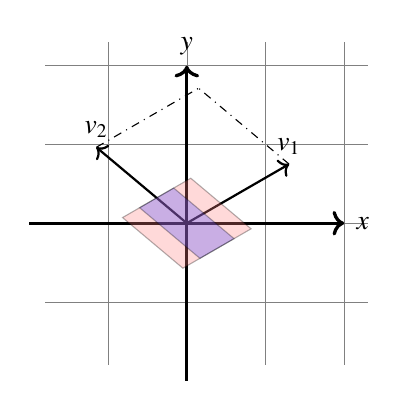
\begin{tikzpicture}
				\draw[style=help lines,step=1cm] (-1.8,-1.8) grid (2.3,2.3);
				
				\draw[->,very thick] (-2,0) -- (2,0) node[right] {$x$};
				\draw[->,very thick] (0,-2) -- (0,2) node[above] {$y$};
				
				\draw[->, thick] (0,0) -- (30:1.5);
				\draw[->, thick] (0,0) -- (140:1.5);
				\draw[dash dot] (30:1.5) -- ++ (140:1.5);
				\draw[dash dot] (140:1.5) -- ++(30:1.5);
				
				
				\filldraw[fill= red!50,opacity=0.3] (30:0.5) -- ++ (140:0.5) -- ++ (210:1) -- ++(-40:1) -- ++(30:1)-- cycle;
				
				\filldraw[fill = blue!70,opacity =0.3] (30:0.25) -- ++(140:0.5) -- ++(210:0.5) -- ++(-40:1) -- ++(30:0.5) -- cycle;
				
				\node[above] at (30:1.5){$v_1$};
				\node[above] at (140:1.5){$v_2$};
			\end{tikzpicture}
		\caption{The red parallelogram is a `ball' centered at origin with radius $\epsilon$ respect to metric $d$; the blue parallelogram is a 	`ball' centered at origin with radius $\epsilon$ respect to metric $d_2$.}
		\end{figure}
		
		In the metric $\tilde{d}_{n+1}$, a ball of radius $\epsilon$ is a parallelogram with side length $2\epsilon |\lambda|^{-n}$ in the $v_1$-direction and $2\epsilon$ in the $v_2$-direction. Indeed, $d_{n+1}(x,y)=\max_{1\leq i\leq n}\{ d(A^ix, A^i y)\}<\epsilon$ Also note that $A^i(x-y)=A^i(a_1v_1+a_2v_2)=\lambda^i a_1 v_1+\lambda^{-i} a_2v_2$ if we assume $x-y=a_1v_1+a_2v_2$. Hence $\max_{1\leq i\leq n}\{|\lambda^i a_1|,|\lambda^{-i}a_2|\}=\max\{|\lambda^n a_1|,|a_2|\}<\epsilon$. We can then obtain the side length. In particular, the Euclidean area of a $\tilde{d}$-ball of radius $\epsilon$ is not greater than $4\epsilon^2|\lambda|^{-n}$. Since the induced metric $d$ on $\T^2$ is locally isometric to $\tilde{d}$, we conclude that for sufficiently small $\epsilon$, the Euclidean area of a $d_n$-ball of radius $\epsilon$ in $\T^2$ is at most $4\epsilon^2 |\lambda|^{-n}$. It follows that the minimal number of balls $d_n$-radius $\epsilon$ needed to cover $\T^2$ is at least $|\lambda|^n/4\epsilon^2$, which is the area of $\T^2$, 1, divided by area of $d_n-\epsilon$ ball. In other words, 
		$$
		\spn(n,\epsilon, A)\geq \frac{|\lambda|^n}{4\epsilon^2}.
		$$
		We have obtained a lower bound of $h(A)$ which is
		$$
		\lim_{\epsilon\to 0^+}\liminf_{n\to\infty} \frac{1}{n}\log \frac{|\lambda|^n}{4\epsilon^2} = \lim_{\epsilon\to 0^+} \log|\lambda|=\log|\lambda|.
		$$
		
		For the upper bound, since the closed $\tilde{d}_n$-balls are parallelograms, there is a tiling of the plane by $\epsilon$-balls whose interiors are disjoint. The Euclidean area of such a ball is $C \epsilon^2 |\lambda|^{-n}$ where $C$ depends on the angle between $v_1$ and $v_2$. For small $\epsilon$, any $\epsilon$-ball that intersects the unit square $[0,1]\times [0,1]$ is entirely contained in the larger square $[-1,2]\times [-1,2]$. Therefore the number of balls that intersect the unit square does not exceed the area of the larger square divided by the area of a $\tilde{d}_n$ ball of radius $\epsilon$. It follows that
		$$
		\spn (n,\epsilon,A)\leq \frac{9\lambda^n}{C\epsilon^2},
		$$
		thus $h(A)\leq \log|\lambda|$.
	\end{proof}
	
	
	\begin{proposition}{Entropy of $E_m$}{Entropy of Em}
		The topological entropy of the expanding map $E_m:S^1\rightarrow S^1$ is $\log m$.
	\end{proposition}
	
	\begin{proof}
		The distance on $S^1$ is $d(x,y)=\min\{|x-y|, 1-|x-y|\}$. Recall that if $d(x,y)<1/2m$, then $d(E_m x, E_m y)=md(x,y)$. Consider $x,y$ is sufficiently close. We can think so since we have to let $\epsilon\to 0^+$ when calculating entropy. With this assumption, we obtain 
		$$
		d_{n+1} (x,y) = \max_{0\leq i\leq n} d(E_m^i x, E_m^i y) = m^{n}d(x,y).
		$$
		Therefore, the $d_{n+1}$ ball with radius $\epsilon$ would have natural length $2\epsilon/m^n = 2m^{-n}\epsilon$. Then consider the closed balls with disjoint interior. Since the geometrical figure is clear (they are all actually intervals), it is clear that the minimal number of $(n+1,2\epsilon)$ balls needed to cover $S^1$ will be 
		$$
		\frac{1}{2m^{-n}\epsilon}\leq \cov (n+1,2\epsilon,E_m)<\frac{1}{2m^{-n}\epsilon}+1.
		$$
		Divided by $n+1$, then taking $\lim\inf_{n\to\infty}$ and $\lim_{\epsilon\to 0^+}$, we get $h(E_m)=\log m$.
	\end{proof}
	
	
	
	
	
	
	\begin{proposition}{Entropy of solenoid}{}
		The topological entropy of the solenoid map $F:S\to S$ is $\log2$.
	\end{proposition}
	
	\begin{proof}
		Recall that $F$ is topologically conjugate to the automorphism $\alpha:\Phi\rightarrow \Phi$, where
		$$
		\Phi = \{(\phi)_{i=0}^{\infty}: \phi_i \in [0,1), \phi_i =2\phi_{i+1} \mod 1\},
		$$
		and $\alpha$ is coordinate-wise multiplication by $2 (\mod 1)$. Thus $h(F)=h(\alpha)$. Define distance on $\Phi$ to be
		$$
		d((\phi),(\phi'))=\sum_{n=1}^{\infty} \frac{1}{2^n} |\phi_n-\phi_n'|,
		$$
		where $|\cdot|$ is the distance on $S^1=[0,1]\mod 1$.
		
		The map $\pi:\Phi \rightarrow S^1$, $(\phi)\mapsto \phi_0$ is a semiconjugacy form $\alpha$ to $E_2$. Hence, $h(\alpha)\geq h(E_2)=\log 2$ (Proposition \ref{prop:Entropy of Em}). We now show that $h(\alpha)\leq \log 2$ by constructing an $(n,\epsilon)$-spanning set.
		
		Fix $\epsilon>0$ and choose $k\in \N$ such that $2^{-k}<\epsilon/2$. For $n\in\N$, let $A_n\subset \Phi$ consists of $2^{n+2k}$ sequences, $\psi^j = (\psi_i^j)$, where $\psi_i^j = j\cdot 2^{-(n+k+i)}\mod 1$, $j=0,\dots, 2^{n+2k}-1$. We claim that $A_n$ is $(n,\epsilon)$-spanning. Let $\phi=(\phi_i)$ be a point in $\Phi$. Choose $j\in \{0,\dots, 2^{n+2k}-1\}$ so that $|\phi_k-j\cdot 2^{-(n+2k)}|\leq 2^{-(n+2k+1)}$. It is easy to see the reason with the help of Figure \ref{fig:S1}. Rigorously speaking, since $\phi_k$ lies in one of the intervals of 
		$$
		[j\cdot 2^{-(n+2k)}, (j+1)\cdot 2^{-(n+2k)}),\quad j\in\{0,\dots, 2^{-(n+2k)}-2\},
		$$
		there must exist such $j$. Then $|\phi_i-\psi_i^j|\leq 2^{k-i}2^{-(n+2k+1)}$ since we have $E_mx$ preserves the distance when $d(E_m x, E_m y)<1/2$. It follows that 
		$$
		d(\alpha^m \phi,\alpha^m \psi^j) = \sum_{i=1}^\infty \frac{|2^m\phi_i - 2^m \psi_i^j|}{2^i}<\sum_{i=0}^k \frac{2^m |\phi_i-\psi_i^j|}{2^i}+\frac{1}{2^k}<2^m \sum_{i=0}^k \frac{2^{k-i}2^{-(n+2k+1)}}{2^i}+\frac{1}{2^k}<\frac{1}{2^{k-1}}<\epsilon,
		$$
		where we use the distance on $S^1$ is no more than $1$.		Thus $d_n(\phi,\psi^j)<\epsilon$, so $A_n$ is $(n,\epsilon)$-spanning. Hence,
		$$
		h(\alpha)\leq \lim_{n\to\infty} \frac{1}{n}\log 2^{n+2k}=\log 2.
		$$
				\begin{figure}
			\centering
			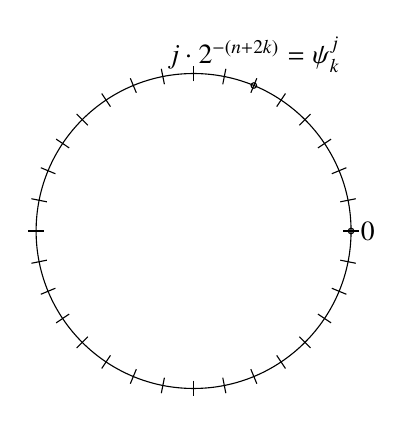
\begin{tikzpicture}
				\draw (0,0) circle (2cm);
				\foreach \x in {0,1, ...,31}
				\draw (11.25*\x:1.9) -- (11.25*\x:2.1);
				\draw (11.25*6:2) circle (1pt) node[above=1pt] {$j\cdot 2^{-(n+2k)}=\psi_k^j$};
				\draw (0:2) circle (1pt) node[anchor=west] {$0$};
			\end{tikzpicture}
			\caption{We can separate $S^1$ into $2^{n+2k}$ pieces with each of length $2^{-(n+2k)}$, here $n=1, k=2$.}\label{fig:S1}
		\end{figure}
	\end{proof}

		
		
		
		
		\begin{proposition}{Solenoid map is expansive}{}
			The solenoid map is expansive. Consequently, $h(F)=h_{\epsilon}(F)$ for $\epsilon$ less than the expansiveness constant (Proposition \ref{prop:entropy with expansive}), which in fact is $1/3$.
		\end{proposition}
		
		\begin{proof}
			\cite{williams1955note}
			Since the solenoid map $F$ is topologically conjugate to the automorphism $\alpha:\Phi\rightarrow \Phi$. It suffices to show $\alpha$ is expansive, i.e. there is a $\delta>0$ such that for any distinct points $\phi,\psi\in \Phi$ there exists $n\in\Z$ such that $d(\alpha^n(\phi),\alpha^n(\psi))>\delta$. Recall the metric in $\Phi$ we used is
			$$
			d(\phi,\psi)=\sum_{n=0}^{\infty}\frac{1}{2^n}|\phi-\psi|.
			$$
			
			There are two cases for distinct points $\phi,\psi$. The first case is that $\phi_i\neq \psi_i$ for each $i\in \N$. The second case is that $\phi_i=\psi_i$ for $i=0,\dots,n-1$, but not equal in $i\geq n$. We can only have those two cases since once $\phi_n=\psi_n$ for some $n$, then $\phi_i=\psi_i$ for $i\leq n$ by the definition of points in $\Phi$. And we cannot conclude $\phi_i=\psi_i$ for $i> n$ since $E_m$ is not invertible, as there might have two preimages.
			
			Now consider case 1, i.e. $\phi_i\neq \psi_i$ for each $i\in\N$. Since $\alpha$ is coordinate-wise multiplication by $2$ (mod 1), consider only the first coordinate $\phi_0$ and $\psi_0$. If $|\phi_0-\psi_0|<1/4$, then $|\alpha(\phi_0)-\alpha(\psi_0)|=2|\phi_0-\psi_0|$. It is expanding, so we must have some $n\in\N\subset\Z$ such that $|\alpha^n(\phi_0)-\alpha^n(\psi_0)|>1/4$. Then $d(\alpha^n(\phi),\alpha^n(\psi))>1/4$.
			
			For the second case, if we iterate backward $n$ times, then 
			$$
			\alpha^{-n}(\phi)=(\phi_n,\phi_{n+1},\dots),\quad \alpha^{-n}(\psi)=(\psi_n,\psi_{n+1},\dots)
			$$
			and $\phi_n\neq \psi_n$. We should have $|\phi_n-\psi_n|=1/2$ since $\phi_{n-1}=2\phi_n=2\psi_n=\psi_{n-1}\mod 1$. Then
			$d(\alpha^{-n}(\phi),\alpha^{-n}(\psi))>1$.
			
			For both cases, $\alpha$ is expansive, so the proof completes.
		\end{proof}
		
		
		
		
		
	
	
	
	
	
	
	
	
	
	
	
	
	

	\section{Ergodic Theory}
	In Topological dynamics, we are interested in every point in the dynamics and the qualitative behavior of it. However, in Ergodic theory, we are interested in the statistical properties of a dynamical system and the behavior of a full-measure set.
	
	\subsection{Measure Theory Preliminaries}
	\newcommand{\frakA}{\mathfrak{A}}
	\begin{definition}{$\sigma-$algebra}{sigma algebra}
		A collection of set $\frakA\subset \{A:A\subset X\}$ is called $\sigma-$algebra if it satisfies:
		\begin{enumerate}
			\item $\frakA\neq \emptyset$;
			\item If $A\in \frakA$, then $X-A\in \frakA$;
			\item If $\{A_n\}_{n\in\N}\subset \frakA$, then 
			$$
			\bigcup_{n\in \N} A_n \in \frakA.
			$$
		\end{enumerate}
	\end{definition}
	
	\begin{proposition}{}{}
		If $\{A_n\}_{n\in\N}\subset \frakA$, then 
		$$
		\bigcap_{n\in \N} A_n \in \frakA.
		$$
		
 	\end{proposition}
	\begin{proof}
		Use the second and third assumption in the definition of $\sigma-$algebra.
	\end{proof}
			\newcommand{\A}{\mathcal{A}}
	Any non-empty family of sets in $2^X$, $\A$, generates a $\sigma-$algebra. We will call it $\frakA(\A)$, the $\sigma-$algebra generated by $\A$. (We haven't defined what is 	`generate', I think it means the span with operators intersections, unions and complements.)
	\begin{definition}{}{}
		Given a set $X$ compact and metric, $\frakA$ a $\sigma-$algebra on $X$. We say a function $\mu: \frakA\rightarrow \mathbb{R}_0^+$ is a \emph{measure} if it is \emph{$\sigma-$additive}, i.e.
		$$
		\mu\left(\bigcup_{n\in \N} A_n\right) = \sum_{n\in\N} \mu(A_n),
		$$
		for any $A_n\in \frakA$.
	\end{definition}
	
	\begin{proposition}{}{}
		$\mu(\emptyset)=0$.
	\end{proposition}

	\newcommand{\B}{\mathfrak{B}}
	
	\begin{definition}{}{}
		\begin{enumerate}
		\item If $\mu (A)=0$, then we call $A$ a \emph{null-set}. If $\mu(X-A)=0$, then $A$ is a \emph{full-measure} set.
		
		\item We say that a measure $\mu$ is \emph{complete}, if $A\subset \frakA$ such that $\mu(A)=0$, then for all $E\subset A$ we have $E\in \frakA$.
		
		\item And if $A\in \frakA$, then $A$ is said to be \emph{measurable}.
		
		\item Given $\frakA$ a $\sigma-$algebra, with $\mu$ measure. $\overline{\frakA}$ is a completion of $\frakA$ if it is the smallest complete $\sigma-$algebra containing $\frakA$. In other words, $\overline{\frakA}$ is the $\sigma$-algebra generated by $\frakA$ and all the subsets of null-sets of $\frakA$.
		\end{enumerate}
	\end{definition}
	\begin{definition}{Measure space}{}
		A \emph{measure space} is the triple $(X,\frakA,\mu)$, where $X$ any set, $\frakA$ is a $\sigma$-algebra, $\mu$ is a measure. 
	\end{definition}
		In the context, we will always assume $\frakA $ is complete and $\frakA$ is $\sigma$-finite, i.e.
		$$
		X=\bigcup_{n\in \N} X_n \quad \mu(X_n)<\infty.
		$$
	\begin{definition}{}{}
		Let $(X,\frakA,\mu)$ and $(Y,\B,\nu)$ be a measure space.
		\begin{enumerate}
			\item If $\mu(X)=1$, then we called the corresponding measure space a \emph{probability space} and $\mu$ is a probability measure. If $\mu'(X)<\infty$ then $\nu(A)=\mu'(A)/\mu'(X)$ will be a probability measure.
			\item The \emph{product measure} is 
			$
			(X\times Y, \frakC, \mu\times \nu)
			$
			where $\frakC$ is the completion of the $\sigma-$algebra generated by the sets of the form $A\times B$ where $A\in \frakA$, $B\in \B$, and $(\mu\times v)(A\times B)=\mu(A)v(B)$.
			\item Let $(X,\frakA,\mu)$ and $(Y,\B,v)$ be a measure space. $T:X\rightarrow Y$ is a \emph{measurable map} if for all $B\in\B$, $T^{-1}(B)\in \frakA$.
			\item A measurable map $T:X\rightarrow Y$ is \emph{non-singular} if $\nu(E)=0$ then $\mu(T^{-1}(E))=0$. The pre-image of a null-set is a null-set.
		\end{enumerate}
	\end{definition}

 
 
 
 
 	\begin{definition}{Measure-preserving and Invariant}{}
 		\begin{enumerate}
 			\item A measurable map $T:X\rightarrow Y$ is \emph{measure-preserving} if $$\mu(T^{-1}(A))=\nu(A)$$ for all $A\in \B$. In particular, for measure $T:X\rightarrow X$, then the definition of measure preserving will be like $$\mu(T^{-1}(A))=\mu(A)$$ for all $A\in \frakA$.
 			\item When a transformation preserves a measure $\mu$, then we say that $\mu$ is \emph{$T$-invariant}.
 		\end{enumerate}
 	\end{definition}
 	The meaning of preserving measure in practical is that when the dynamic transformation $T$ acts on some subset of $X$, then the volume of the subset won't change. See the informal explanation in the beginning of section \ref{sec:ergodic}. 
 	\begin{example}{Lebesgue measure is invariant under $E_2$}{}
 		The Lebesgue measure on the unit interval $[0,1]$ is invariant under the $E_2$ transformation, where $E_2$ is the doubling map defined on $S^1$, i.e. $E_2:x\mapsto 2x \mod 1$.
 	\end{example}
 	\begin{proof}
 		It suffices to prove that the measure of any interval is the same as the measure of the preimage of the inverval under $E_2$. Indeed, consider a measurable subset $A$ of $[0,1]$. The first one of Littlewood's three principles (cf. Chapter 1, Section 4.3 in \cite{Stein:1385521}) says that every set is nearly a finite union of intervals. Formally, we have the following theorem (cf. Chapter 1, Theorem 3.4 in \cite{Stein:1385521}): 
 		\begin{quote}
 			Suppose $E$ is measurable subset of $\R^d$ with finite measure. Then for every $\epsilon>0$ there exists a finite union $F=\bigcup_{j=1}^N Q_j$ of closed cubes such that $m(E\bigtriangleup F)\leq \epsilon$. 
 		\end{quote}
 		In our case, we can assume without loss of generality that $I=\bigcup_{j=1}^N I_j$ with $I_j$ almost disjoint intervals that satisfies $m(A\bigtriangleup I)\leq \epsilon$. If $m(E^{-1}_2 I_j)=m(I_j)$ for all $j$ then 
 		$$
 		m(E_2^{-1} (I))=m(E_2^{-1}(\bigcup_{j=1}^N I_j))=m(\bigcup_{j=1}^N E_2^{-1}(I_j))=\sum_{j=1}^N m(E_2^{-1}(I_j))=\sum_{j=1}^N m(I_j)=m(I).
 		$$
 		Therefore
 		$$
 		m(E_2^{-1}(A))=m(E_2^{-1}(I))+m(E_2^{-1}(A-I))=m(I)+m(E_2^{-1}(A-I))=m(A)-m(A-I)+m(E_2^{-1}(A-I)).
 		$$
 		
 		Now consider $I=[a,b]$, with $m(I)=b-a$. We have $E_m^{-1}(I)=[\frac{a}{2},\frac{b}{2}]\cup [\frac{a+1}{2},\frac{b+1}{2}]$ so that $E_m^{-1}(I)=\frac{b-a}{2}+\frac{b-a}{2}=b-a$. The proof is complete.
 	\end{proof}
 
 		\newcommand{\one}{\mathbf{1}}
 
 	\begin{lemma}{Invariant of integral}{invariant of integral}
 		$T$ is measure preserving if and only if for each $f\in L^1 (X,\frakA,\mu)$, we have
 		$$
 		\int f d\mu=\int f\circ Td\mu.
 		$$
 	\end{lemma}
 	\begin{proof}
 		First note that for $A\in\frakA$, $\one_A\in L^1(X,\frakA,\mu)$ and $\one_A\circ T=\one_{T^{-1}A}$. The latter is because they both equal $1$ if $Tx\in A$ and equal $0$ otherwise. 
 		
 		Assume $T$ is measure preserving, then $\mu(A)=\mu(T^{-1}(A))$ for $A\in \frakA$, so that
 		$$
 		\int \one_A d\mu=\mu(A)=\mu(T^{-1}(A))=\int \one_{T^{-1}(A)} d\mu =\int \one_A\circ Td\mu.
 		$$
 		Hence we prove the result for simple functions. And then for any $f\in L^1(X,\frakA,\mu)$, we can find an increasing sequence of simple functions $f_n$ with $f_n\to f$ as $n\to \infty$. For each $n$ we have
 		$$
 		\int f_n d\mu =\int f_n \circ T d\mu,
 		$$
 		then applying Monotone Convergence Theorem to both sides, we get
 		$$
 		\int fd\mu=\int f\circ T d\mu.
 		$$
 		Then for general real-valued $f$, consider $f=f^{+} - f^{-}$, we have
 		$$
 		\int f d\mu= \int f^{+}- f^{-}d\mu=\int f^{+}\circ T-f^{-}\circ Td\mu=\int f\circ Td\mu,
 		$$
 		which completes the proof of the first part.
 		
 		Conversely, just let $f=\one_A$, then
 		$$
 		\mu(A)=\int \one_Ad\mu =\int \one_A \circ Td\mu=\int \one_{T^{-1}(A)}=\mu(T^{-1}(A)).
 		$$
 	\end{proof}
 	This lemma is very useful. Let us see an example using it.
 	
 	\begin{example}{}{}
 		Let $T$ be a measure-preserving transformation of $(X,\frakA,\mu)$, and let $f\in L^1(X,\mu)$ satisfy $f(T(x))\leq f(x)$ for a.e. x. Then $f(T(x))=f(x)$ for a.e. x.
 	\end{example}
 	We will see later that $f$ is called essentially $T$-invariant function.
 	\begin{proof}
 		Assume that the set of $x$ such that $f(T(x))<f(x)$ has positive measure. Therefore we must have
 		$$
 		\int fT d\mu <\int fd\mu,
 		$$
 		which contradicts with the lemma.
 	\end{proof}
 
 
 	\begin{lemma}{}{}
 		If $T$ is a invertible, measurable transformation and $T^{-1}$ measurable and non-singular then $\{T^n\}_{n\in \Z}$ forms a group of measurable transformation.
	\end{lemma}
	We need the assumption `non-singular' because in principle, an injective transformation could be singular. For instance, we could have an \emph{atom}, i.e. $x\in X$ and $\mu(\{x\})>0$, and also $\mu(\{Tx\})=0$. Then we would have the singular property for $E=\{Tx\}$.
	\begin{definition}{Isomorphic, automorphism and extension}{}
		\begin{enumerate}
			\item Two measure spaces, $(X,\frakA,\mu)$, $(Y,\B,\nu)$ are \emph{isomorphic} if there exists full set $X'\subset X$, full set $Y'\subset Y$ and $T:X'\rightarrow Y'$ bijection such that $T, T^{-1}$ are measurable and measure preserving.
			\item An isomorphism $T:(X,\frakA,\mu)\rightarrow (X,\frakA,\mu)$ is called \emph{automorphism}.
			\item Let $T$ and $S$ be measure preserving transformation of $(X,\frakA,\mu)$ and $(Y,\B,\mu)$. $T$ is an \emph{extension} of $S$, if there exits full set $X'\subset X$ and full set $Y'\subset Y$, and exists a measure preserving map $\psi: X'\rightarrow Y'$ satisfying $\psi \circ T = S\circ \psi$. If $\psi$ is an isomorphism, then $T,S$ are \emph{isomorphic}.
			\begin{tikzcd}
				&X' \arrow[r, swap, "T"] \arrow[d, "\psi"] &X' \arrow[d, swap, "\psi"] \\
				&Y' \arrow[r, "S"]  &Y'
			\end{tikzcd}
		\end{enumerate}
	\end{definition}
	Later we will define a measure $\mu$ on $(\Sigma^n, \sigma).$ In dynamical systems, any transformation isomorphic to $\sigma$ is call \emph{Bernoulli}.
	
	In particular, the product of two measure sets is an extension of either of the two sets.
	
	\subsection{Interaction of measures and topologies}
	\begin{definition}{Borel $\sigma$-algebra and Borel measure}{}
		\begin{enumerate}
			\item Let $X$ be a topological space, $(X,d)$ a compact metric space. The \emph{Borel $\sigma$-algebra} is the smallest $\sigma$-algebra containing all open sets of $X$. 
			\item If $\B$ is the Borel $\sigma$-algebra, then a measure $\mu$ called a \emph{Borel measure} if $\mu(K)<\infty$ for all $K$ compact.
		\end{enumerate}
	\end{definition}

	
	\begin{proposition}{}{}
		A Borel measure is always regular, i.e. for all $A\in\B$, $\mu(A)=\inf\{\mu(U): U\text{ open, } A\subset U\}$, $\mu(A)=\sup\{\mu(K): K\text{ compact, } K\subset A\}$. In particular, for all $A\in\B$, there exists $K\subset A \subset U$ such that for all $\epsilon>0$, $\mu(U-K)<\epsilon$.
	\end{proposition}
	
	\begin{definition}{}{}
		A finite measure space is called a \emph{Lebesgue space} if it is isomorphic to the union of an interval $[0,a]$(with the Lebesgue measure) and at most countably many atoms.
	\end{definition}

	\begin{lemma}{}{}
		For a separable complete metric space $X$, define finite Borel measure on $X$, $\frakA$ be the completion of the Borel $\sigma$-algebra w.r.t $\mu$. Then $(X,\frakA, \mu)$ is a Lebesgue space. 
		
		In particular, $[0,1]^2$ in the Lebesgue measure is isomorphic to $[0,1]$.
	\end{lemma}
	\begin{definition}{}{}
		A Lebesgue space with no atoms is called \emph{non-atomic} and it is always isomorphic to $([0,1],m)$, where $m$ is the Lebesgue measure.
	\end{definition}
	
	\begin{definition}{}{}
		Let $(X,\B,\mu)$ be a measure space. A property holds \emph{mod 0} in $X$ or $\mu-$ almost everywhere or $\mu$-a.e. $x$ if the property holds on a full measure set.
	\end{definition}

	\begin{example}{Not proven yet}{}
		The hyperbolic automorphism $A:\T^2\rightarrow \T^2$, with $A=\begin{pmatrix}
			2 & 1\\
			1 & 1
		\end{pmatrix}$ is dense almost every orbit.
	\end{example}
	
	\begin{definition}{}{}
		Let $(X,\B,\mu)$ be a measure space. Two measurable functions are \emph{equivalent} if they coincide mod 0.
	\end{definition}
	\begin{example}{}{}
		$f(x)=\begin{cases}
			1  \quad &x\in \mathbb{Q}\\
			0 &  x\notin \mathbb{Q}
		\end{cases}$
	on $[0,1]$ is equivalent to $0$.
	\end{example}
	\begin{proof}
		Since they are equal besides a set of measure 0.
	\end{proof}
	
	\subsection{Space of Functions}
	
	\begin{definition}{$L^p$ space}{}
		For $p\in (0,\infty)$ the space $L^p(X,\mu)$ is the set of equivalent classes mod 0  of measure functions $f:X\rightarrow \mathbb{C}$ such that
		$$
		\int_X |f|^p d\mu <\infty
		$$
		For $p>1$, the norm is defined to be $\|f\|_p=\left(	\int_X |f|^p d\mu\right)^{1/p}$.
	\end{definition}
	
	Recall that $L^2(X,\mu)$ is a Hilbert space $(f,g)_2=\int_X f\overline{g}d\mu$. $L^\infty(X,\mu)$ is a space of essentially bounded functions and $\|f\|_{\infty}=\text{ess}\sup_X|f|$. Essentially means we do not consider set of measure 0.
	
	\begin{proposition}{}{bounded function is integrable}
		If $\mu$ finite, then $L^{\infty}\subset L^p$ for all $p>0$.
	\end{proposition}
	
	
	\begin{definition}{}{}
		The continuous functions $f:X\rightarrow \mathbb{C}$ with compact support, denoted by $C_0(X,\mu)$ if there exists $K\subset X$ compact set such that $f(x)=0$ outside $K$.
	\end{definition}
	
	\begin{proposition}{}{}
		$C_0(X,\mu)$ is dense in $L^p(X,\mu)$ for all $p>0$.
	\end{proposition}

	\subsection{Recurrence}

	\begin{theorem}{Poincare Recurrence Theorem}{}
		Let $(X,\B,\mu)$ be a probability measure space,  $T:X\rightarrow X$ be measure preserving. If $A$ measurable set, then for $\mu$-a.e. $x\in A$ there exists $n\in\N$ such that $T^n(x)\in A$. Moreover, a.e. $x\in A$, there exists infinitely many $k\in \N$ such that $T^k(x)\in A$.
	\end{theorem}

	\begin{proof}
		Let $B=\{x\in A: T^n(x)\notin A,\forall n\in\N\}$, which is the points that never return to $A$. Note that
		\begin{align*}
			B&=\{x\in A: x\notin T^{-n}(A),\forall n\in\N\}=\{x\in A: x\in [T^{-n}(A)]^c,\forall n\in\N\}\\
			&=\{x\in A: x\in \bigcap_{n\in \N}[T^{-n}(A)]^c \}=\left\{x\in A: x\in\left[\bigcup_{n\in \N}T^{-n}(A)\right]^c\right\}\\
			&=A-\bigcup_{n\in \N}T^{-n}(A).
		\end{align*}
	Claim that all preimages of $B$ are 2 by 2 disjoint. It is enough to prove $B\cap T^{-j}(B)=\emptyset$ for all $j\in\N$, since
	$$
	T^{-k}(B)\cap T^{-j}(B)=T^{-k}(B\cap T^{-j+k}(B)).
	$$
	Now note that
	\begin{align*}
		B\cap T^{-j}(B)=&\left(A-\bigcup_{n\in \N} T^{-n}(A)\right)\cap T^{-j}(A-\bigcup_{n\in \N}T^{-n}(A))\\
		=& \left(A-\bigcup_{n\in \N} T^{-n}(A)\right)\cap T^{-j}(A)=\emptyset.
	\end{align*}
	However, we then have
	$$
	\mu\left(\bigcup_{j\in \N}T^{-j}(B)\right)=\sum_{j\in\N} \mu(T^{-j}(B))=\sum_{j\in\N}\mu(B)\leq \mu(X)=1.
	$$
	So we must have $\mu(B)=0$. In other words, for $x\in A-B$, or almost every $x$, there exists $n\in\N$ such that $T^n(x)\in A$.
	
	Now define $C=\{x\in A:\exists n\in\N, T^k(x)\notin A \forall k\geq n\}$, the set of points in $A$ that return to $A$ only finite number of times. We want to prove $\mu(C)=0$. We will complete proof similarly. Note that in fact as what we done previously
	$$
	C=\bigcup_{n\in \N}\left[A-\bigcup_{k\geq n}T^{-k}(A)\right].
	$$
	Let $C_n = A-\bigcup_{k\geq n}T^{-k}(A)$. Then it suffices to show $\mu(C_n)=0$. It is clear that $C_n\in \B$. Rewrite $C_n$ as
	$$
	C_n = A-\bigcup_{k\geq n}T^{-k}(A)\subset \bigcup_{k\geq 0}T^{-k}(A)-\bigcup_{k\geq n}T^{-k}(A).
	$$
	So that
	$$
	\mu(C_n)\leq \mu\left(\bigcup_{k\geq 0}T^{-k}(A)\right)-\mu\left(\bigcup_{k\geq n}T^{-k}(A)\right)=0
	$$
	since $T^{-n}\left(\bigcup_{k\geq 0}T^{-k}(A)\right)=\left(\bigcup_{k\geq n}T^{-k}(A)\right)$. This ends the proof.
	\end{proof}
	We give an example to show that Poincare Recurrence Theorem fails if $\mu(X)=\infty$. Take $X=\R$, $\mu$ be the Lebesgue measure. $T(x)=x+1$ of course measure preserving. However for example points in $A=[0,1/2]$ will never return, i.e. $T^{-j}(A)\cap A=\emptyset$ for $j\geq 1$.

	We have previously defined another type of (forward) recurrence, which is $x\in \omega(x)$. We will see later that for a (finite) Borel measure there is a relationship between two notions. 
	
	\newcommand{\supp}{\text{supp}}
	\begin{definition}{Support of measure}{support}
		Let $X$ be a compact metric space, $\mu$ a Borel measure on $X$. The \emph{support of $\mu$} is the set
		$$
		\supp(\mu) = \{x\in X: \mu(B(x,\epsilon))>0,\forall \epsilon>0\}.
		$$
	\end{definition}

	\begin{proposition}{}{}
		The support measure $\supp(\mu)$ is closed.
	\end{proposition}
	
	\begin{proof}
		Consider a convergent sequence $x_n\in \supp(\mu)$ with $x_n\to x$. For any $\epsilon>0$, there exists $N$ such that $x_N\in B(x,\epsilon)$. Since $B(x,\epsilon)$ is open, there is a open ball centered at $x_N$, $B(x_N, \delta)\subset B(x,\epsilon)$. By assumption, $\mu(B(x_N, \delta))>0$, and thus $\mu(B(x,\epsilon))>0$, i.e. $x\in \supp(\mu)$, which shows $\supp(\mu)$ is closed.
	\end{proof}
	
	\begin{proposition}{}{support}
		\begin{enumerate}
			\item $\supp(\mu)$ is the intersection of all closed full measure set.
			\item $\supp(\mu)$ is the complement of the union of all open null measure set.
		\end{enumerate}
	\end{proposition}

	\begin{proof}
		It is enough to prove the first one, just noting that
		$$
		\left(\bigcup_i U_i\right)^c=\left(\bigcup_i F^c_i\right)^c=\bigcap_i F_i.
		$$
		To prove it, first, we have to prove for each $x\in \supp(\mu)$, $x\in F$ once $F$ is a closed full measure set. If not, $x\in F^c$ with $F^c$ open and null measure, it contradict with $x\in \supp(\mu)$. Second, we have to prove if $x\in F$ for any $F$ closed full measure set, then $x\in \supp(\mu)$. If not, then for some $x_0\in F_i$, $\mu(B(x_0,\epsilon_0))=0$ for some $\epsilon$. $x_0$ will not be in the closed full measure set of $F_i-B(x_0,\epsilon_0)$, contradiction.
	\end{proof}

	\begin{proposition}{}{}
		$X$ compact metric space, $\mu$ Borel probability measure on $X$. $T:X\rightarrow X$ continuous transformation which is measure preserving. Then a.e. $x$ is recurrent ($x\in \omega(x)$). This implies $\supp(\mu)\subset \overline{R(T)}$.
	\end{proposition}
	\begin{proof}
		Since $X$ is a compact metric space, so there exists an open countable basis $\{U_i\}_{i\in\N}$, i.e. for any $U\subset X$ open set, there exists a subsequence $\{i_n\}$ such that $U= \bigcup_{i_n}U_{i_n}$. By the Poincare Recurrence Theorem there exists a full measure set $\tilde{U}_i$ in $U_i$ such that for all $x\in \tilde{U}_i$, there exists $n_i$ with $T^{n_i}(x)\in U_i$. Let $X_i = (X-U_i)\cup \tilde{U}_i$. Then $\mu(X_i)=1$, i.e. $X_i$ is a full measure set of $X$. Consequently, denote $\tilde{X}=\bigcap_{i=1}^{\infty} X_i$, then it also has full measure by sub-additivity. We want to prove that all the point in $\tilde{X}$ is recurrent. For each $x\in \tilde{X}$, let $i_n(x)$ be a subsequence of $i$ depends on $x$ such that $U_{i_{n+1}(x)}\subset U_{i_n(x)}$ and $\bigcap_{n\in\N}U_{i_{n}(x)}=\{x\}$. So there exists $N_{i_{n}(x)}\in \N$ such that $T^{N_{i_{n}(x)}}(x)\in U_{i_n(x)}$. Let $n\to \infty$, $T^{N_{i_{n}(x)}}(x)\to x$, which shows $x\in\tilde{X}$ is recurrent. 
		
		Note that 
		$$
		1=\mu(\tilde{X})=\mu(R(T))=\mu(\overline{R(T)}),
		$$
		so $\overline{R(T)}$ has full measure and closed. Then by Proposition \ref{prop:support}, we know that $\supp(\mu)\subset \overline{R(T)}$.
	\end{proof}
	
	
	
	\subsection{Ergodicity and Mixing}\label{sec:ergodic}
%	Let $X$ be a compact metric space, $T:X\rightarrow X$ dynamical system. $T$ deduces an action over the set of functions $L^2(X,\mu)$. The action is $T*\phi(x)=\phi\circ T(x)$. How independent are the iterates of actions $T$? We shall define the dependence is strong if $T*\phi=\phi$. The independence is strong if $(T*\phi,\phi)=0$. And if $T$ is measure preserving, the strong independence implies $(T^j*\phi,T^k*\phi)=0$.
	
	Before definition, we shall introduce a informal explanation of how those abstract definitions came \cite{enwiki:1086512997}. 
	
	Consider a measure-preserving dynamical system, written $(X,\frakA,\mu, T)$. The set $X$ is understood to be the total space to be filled, for example, the smoke-filled room, a long river, etc. The measure $\mu$ is understood to define the natural volume of the space $X$ and of its subspace. The collection of subspaces is denoted by $\frakA$ (formally, it is the collection of measurable sets which satisfies certain conditions, cf. Definition \ref{def:sigma algebra}) so that for any given set $A\subset X$, the volume of it is $\mu(A)$ (we will explain later when the measure is probability measure). 
	
	The time evolution of the system is describe by a map $T:X\rightarrow X$. Given some subset $A\subset X$, its map $T(A)$ will in general be a deformed version of $A$: it is squashed or stretched, folded or cut into pieces, for example, the horseshoe map. The set $T(A)$ must have the same volume as $A$. Such map is natural in practical since stretching and folding will not change the volume of a object (noodles, for example in horseshoe). And such map is called \emph{measure preserving} map. However, a formal difficulty arises when one tries to reconcile the volume of sets with the need to preserve their size under $T$. That is because, in general (when the map is not invertible), several different points in the domain of a function would map into the same point in its range, i.e. there may be $x\neq y$ but $T(x)=T(y)$. But if we consider the inverse map $T^{-1}: \frakA\to \frakA$, one can find that this inverse map can capture all the points since there won't be a point in the domain that have two images. In other words, it will not lose track of where things came from. Therefore, the proper definition of a measure-preserving map is $\mu(A)=\mu(T^{-1}(A))$.
	
	Our interest now is the time evolution of the system. If a set $A\in \frakA$ eventually comes to fill all of $X$ over a long period of time(that is, if $T^n(A)$ approaches all of $X$ for large $n$), the system is said to be \emph{ergodic}. If every set $A$ behaves in this way, the system is a \emph{conservative system}. On the contrary, if some subsets wander away, so that $T^n(A)$ won't come back to $A$ thus won't approach all of $X$, then it is a \emph{dissipative system}. An example would be water running downhill: once it's run down, it will never come back up again. The lake that forms at the bottom of this river can, however, well-mixed. The ergodic decomposition theorem states that every ergodic system can be split into two parts: the conservative part and the dissipative part.
	
	Mixing is a stronger statement than ergodicity. Mixing asks for this ergodic property to hold between any two sets $A$ and $B$, not just between $A$ and $X$. That is, given two sets $A,B\in \frakA$, a system is said to be topologically mixing if there is an integer $N$ such that, for all $n>N$, one has $T^n(A)\cap B\neq \emptyset$.
	
	The above discussion appeals to a physical sense of a volume in 3-D. Now we go to the abstract space with the probability measure, $\mu(X)=1$, or equivalently, finite measure (However, the following definitions are available in measure space, rather than finite measure space).
	
		
	Take the fish in the lake as an example. Suppose $X$ is the whole lake, $A$ is a subspace of the lake, the measure $\mu(A)$ is the proportion of fish in the subset $A$. And $T$ a measure preserving transformation. Here measure preserving means that no fish would be dead or born. Then the condition of mixing says that as time goes by, the fish in $A$ must be well-mixed in the lake. However, the ergodicity only ask the fish to approach all of the lake when time goes to infinity, the fish might swan in group without mixing (the $N$ may not exist such that for all $n>N$, $T^n(A)\cap B\neq \emptyset$, but we will have the trace of almost every fish will be dense in the lake, see Proposition \ref{prop:topological consequence}).
	
	\begin{definition}{Essentially $T$-invariant of both functions and sets}{}
		$T:X\rightarrow X$ measure preserving transformation. $f:X\rightarrow \R$ is a measurable function is \emph{essentially $T$-invariant} if $T_* f=f$ a.e, in other words, 
		$$
		\mu(\{x\in X: f(T(x))\neq f(x)\})=0.
		$$
		
		A measurable set $A$ is \emph{essentially $T$-invariant} if its characteristic function $\one_A$ is essentially $T$-invariant. Equivalently, if $\mu(T^{-1}(A)\bigtriangleup A)=0$.
	\end{definition}

	\begin{proof}[Proof of the equivalence]
		The proof is trivial. Just note that 
		\begin{align*}
				&\{x\in X: \one_A(T(x))\neq \one_A(x)\}\\
				=&\{x\in X:\one_A(T(x))=1, \one_A(x)=0\}\cup\{x\in X:\one_A(T(x))=0, \one_A(x)=1\}\\
				=&\{x\in X: T(x)\in A, x\notin A\}\cup \{x\in X: T(x)\notin A, x\in A\}\\
				=&(T^{-1}(A)-A)\cup (A-T^{-1}(A))\\
				=&T^{-1}(A)\bigtriangleup A.
		\end{align*}
	\end{proof}

	\begin{proposition}{Another equivalent definition}{}
		A measurable function $f$ is essentially $T$-invariant if and only if $f(T^n(x))=f$ a.e.. A measurable set $A$ is measure preserving if and only if $\mu(T^{-n}(A)\bigtriangleup A)=0$.
	\end{proposition}
	\begin{proof}
		The second statement is a consequence of the first statement. To prove the first one, note that 
		\begin{align*}
			0=&\mu(\{x\in X: f(T(x))\neq f(x)\}=\mu(T^{-1}\{x\in X: f(T(x))\neq f(x)\})\\
			= & \mu(\{y\in X:f(T^2(y))\neq f(T(y))\}).
		\end{align*}
		This means that $fT^2=fT$ a.e. If $\mathcal{A}$ is complete then the a.e. property is transitive, so that $fT^2=fT=f$ a.e. Then by induction, one can show that $fT^n=fT^{n-1}=\dots=f$ a.e.
	\end{proof}


	\begin{definition}{Ergodicity}{}
		A measure preserving transformation $T:X\rightarrow X$ is \emph{ergodic} if every essentially $T$-invariant set is full or null measure, i.e. if a subset $A\subset X$ satisfies $\mu(T^{-1}(A)\bigtriangleup A)=0$, then either $\mu(A)=0$ or $\mu(A)=\mu(X)$. Equivalently, $T$ is ergodic if any essentially $T$-invariant measurable function is constant$\mod 0$.
	\end{definition}
	
	\begin{proof}[Proof of the equivalence]
		One side is trivial. If we assume any essentially $T$-invariant measurable function is constant$\mod 0$, then for any essentially $T$-invariant set $A$, the characteristic function $\one_A$ is constant$\mod 0$, since the definition says that $\one_A$ is essentially $T$-invariant function. That is, $A$ is either of full measure or null measure.
		
		For the other side, assume that any essentially $T$-invariant set is full or null measure. Then consider an essentially invariant function $\phi$, we want to prove it is constant$\mod 0$. Consider the set $\{\phi(x)>c\}$. This set is obviously essentially $T$-invariant, since $\phi$ is an essentially invariant function (the difference after the action $T$ is of measure zero). Therefore, $\mu(\{\phi(x)>c\})$ is of either full or null measure. Symmetrically, $\{\phi(x)<c\}$ is also of full or null measure. So that $\mu(\{\phi(x)=c\})$ is of full or null measure for all $c$. Since for each $c$, the set is disjoint, there is only one $c$ that has full measure. This shows that $\phi$ is constant $\mod0$. 
	\end{proof}
	
	\begin{proposition}{}{equiv of ergodic}
		Let $T$ be a measure-preserving transformation on a finite measure space $(X,\frakA,\mu)$, and let $p\in (0,\infty]$. Then $T$ is ergodic if and only if every essentially invariant function $f\in L^p(X,\mu)$ is constant $\mod 0$.
	\end{proposition}
	\begin{proof}
		One side is trivial. Assume $T$ is ergodic, then by definition, every essentially invariant function is constant $\mod 0$. 
		
		To prove the converse, let $f$ be an essentially invariant measurable function on $X$, we want to show that $f$ is constant $\mod 0$. Consider for every $M>0$ the function, 
		$$
		f_M(x)=\begin{cases}
			f(x) ,& |f(x)|\leq M\\
			0 ,& |f(x)|>M
		\end{cases}.
		$$
		This function is clearly bounded by $M$ and essentially invariant. Therefore, $f_M(x)\in L^\infty (X,\mu)\subset L^p(X,\mu)$ (cf. Proposition \ref{prop:bounded function is integrable}). By assumption $f_M(x)$ is constant $\mod 0$, for all $M>0$. It follows that $f$ is constant $\mod 0$.
	\end{proof}
	This proposition loose the definition of ergodicity from the set of all essentially invariant measure function to all essentially invariant $L^p$ measurable function, for some $p\in (0,\infty]$.
	
	\begin{proposition}{}{}
		Let $(X,\frakA,\mu)$ be a measure space, and suppose that $f:X\rightarrow \R$ is essentially invariant for a measurable transformation $T$ on $X$. Then there is a strictly invariant measurable function $\tilde{f}$ such that $f(x)=\tilde{f}(x)\mod 0$.
	\end{proposition}
	\begin{proof}
		Consider the full measure set 
		$$
		A=\{x\in X:f(T^n(x))=f(x)\}.
		$$
		We define $\tilde{f}$ to be 
		$$
		\tilde{f}(x)=\begin{cases}
			f(x), & \text{if $x\in A$}\\
			0, & \text{if $x\notin A$}.
		\end{cases}
		$$
		Then $\tilde{f}(x)=f(x)\mod 0$ clearly. And $\tilde{f}(T(x))=f(T(x))=f(x)$ since $T(x)\in A$, so that $\tilde{f}$ is strictly $T$-invariant.
	\end{proof}
	The strict $T$-invariant function is exactly the original function but defined on the full measure set that makes $f$ be invariant.
	
	
	\begin{definition}{(Strong) mixing}{}
		A measure-preserving transformation $T$ on a probability space $(X,\frakA,\mu)$ is called \emph{(strong) mixing} if 
		$$
		\lim_{n\to \infty} \mu(T^{-n}(A)\cap B)=\mu(A)\cdot \mu (B)
		$$
		for any two measurable sets $A,B\in\frakA$.
	%	Equivalently, $T$ is mixing if 
	%	$$
	%	\lim_{t\to \infty} \int_{X} f(T^t(x))\cdot g(x)d\mu=\int_X f(x)d\mu\cdot \int_X g(x)d\mu,
	%	$$
	%	for any bounded measurable functions $f,g$.
	\end{definition}
	The definition is actually meaning that the fish that goes from $A$ to $B$ when the time is large is exactly determined by the initial amount of fish in $A$ and $B$. The assumption of measure-preserving of $T$ means that the total number of fish in any subset of the lake won't change.
	
	\begin{definition}{Weak mixing}{}
		A measure-preserving transformation $T$ of a probability space $(X,\frakA,\mu)$ is called \emph{weak mixing} if for all $A,B\in \frakA$,
		$$
		\lim_{n\to \infty}\frac{1}{n}\sum_{i=0}^{n-1} |\mu(T^{-i}(A)\cap B)-\mu(A)\mu(B)|=0.
		$$
	\end{definition}
	The definition means that the fish in the lake may not be mixed such well, but when we average on time, they can be viewed as mixed well.
	
	\begin{proposition}{}{}
		Mixing implies weak mixing, and weak mixing implies ergodicity.
	\end{proposition}
	\begin{proof}
		Mixing implies weak mixing is followed immediately by Stolz's Theorem. And if $T$ is weak mixing, assume $A$ is essentially invariant measurable set, i.e. $\mu(T^{-n}(A)\bigtriangleup A)=0$, then $\mu(T^{-i}(A)\cap A)=\mu(A)$, so that
		$\mu(A)=\mu(A)^2$ and thus $ \mu(A)=0\text{ or }1.$
	\end{proof}
	
	
	\begin{proposition}{Topological Consequences}{topological consequence}
		Let $X$ be a compact metric space, $T:X\rightarrow X$ a continuous map, and $\mu$ a $T$-invariant Borel measure on $X$. Then
		\begin{enumerate}
			\item If $T$ is ergodic, then the orbit of $\mu$-almost every point is dense in $\supp(\mu)$.
			\item If $T$ is mixing, then $T$ is topologically mixing on $\supp(\mu)$.
		\end{enumerate}
	\end{proposition}
	\begin{proof}
		For the first one, suppose $T$ is ergodic. Let $U$ be a non-empty open set in $\supp(\mu)$. By the definition of support (cf. Definition \ref{def:support}), $\mu(U)>0$. Consider the set that whose forward orbits would be in $U$, namely
		$B=\bigcup_{i\in \N}T^{-n}(U)$. We claim that $B$ is of full measure. To see this, note that $B$ is an essentially $T$-invariant set and by ergodicity, $B$ is either of full or null measure, however, $B$ contains $U$, so we must have $B$ is of full measure. The reason that $B$ is an essentially $T$-invariant set is that since $T^{-1}(B)\subset B$, then $$\mu(T^{-1}(B)\bigtriangleup B)=\mu(B)-\mu(T^{-1}(B))=0$$ for $T$ is measure preserving. Now we have $B$ is of full measure and $B$ is the set whose forward orbits are in $U$. Since $\supp(\mu)$ is a compact metric space, there exists a countable open basis $\{U_k\}_{k\in \N}$. For each $k$, we have the corresponding $B_k$. Now consider $B^*=\bigcap_{k\in\N} B_k$. Since each $B_k$ is of full measure, then $B^*$ is of full measure. And each point in $B^*$ has forward orbits in every $U_k$, which shows that the forward orbits are dense in $\supp(\mu)$.
		
		For the second one, assume $T$ is mixing, then by definition, given any $\epsilon>0$, there exists $N\in\N$ such that for $n>N$,
		$$
		|\mu(T^{-n}(A)\cap B)-\mu(A)\mu(B)|<\epsilon,
		$$
		for any $A,B\subset \supp(\mu)$. Since $A,B\subset \supp(\mu)$, we have $\mu(A)\mu(B)>0$, which implies $\mu(T^{-n}(A)\cap B)>0$ for $n>N$ for some large $N$. Therefore $T^{-n}(A)\cap B\neq \emptyset$. For $x\in T^{-n}(A)\cap B$, $T^nx\in A\cap T^{n}(B)$, i.e. $T$ is topologically mixing on $\supp(\mu)$.
	\end{proof}
	
	
	\newcommand{\C}{\mathbb{C}}
	\subsection{Examples of Ergodicity and Mixing}
	\begin{proposition}{Circle rotation}{}
		The circle rotation $R_{\alpha}$ is ergodic with respect to Lebesgue measure if and only if $\alpha$ is irrational.
	\end{proposition}
	\begin{proof}
		If $\alpha$ is rational then $R_\alpha$ can not be ergodic since the orbit of $x$, say $\{R_\alpha^n(x)\}_{n=1}^N$, is finite but the union of $\epsilon$-ball centered at each point in the orbit is strictly $T$-invariant. But this set is neither full nor null measure.
		
		Suppose $\alpha$ is irrational. By Proposition \ref{prop:equiv of ergodic}, it is enough to prove that any bounded $R_\alpha$-invariant function $f:S^1\rightarrow \C$ is constant$\mod 0$. Since $f\in L^2$, the Fourier series $\sum_{n=-\infty}^{\infty}a_n e^{2n\pi i x}$ of $f$ converges to $f$ in $L^2$ norm. And also $f\circ R_\alpha=\sum_{n=-\infty}^{\infty}a_n e^{2n\pi i (x+\alpha)}$. If $f$ is $R_\alpha$-invariant function, by the uniqueness of Fourier coefficients, 
		$a_n=a_n e^{2n\pi i \alpha}$ for all $n\in\Z$. Since $e^{2n \pi i \alpha}\neq 1$ for $n\neq 0$, we have $a_n=0$ for $n\neq 0$. Thus $f$ is constant$\mod 0$.
	\end{proof}
	
	
	\begin{proposition}{Expanding endomorphism}{}
		An expanding endomorphism $E_m:S^1\rightarrow S^1$ is mixing with respect to Lebesgue measure. 
	\end{proposition}
	\begin{proof}
		Since any measurable subsets of $S^1$ can be approximated by a finite union of intervals of the form $[p/m^i,(p+1)/m^i]$, $p\in\{0,\dots,m^i-1\}$ (this is because firstly Littlewood's Principle says any measurable subsets can be approximated by a finite union of disjoint intervals and secondly each intervals can be approximated by disjoint intervals of such form), so it is sufficient to consider two intervals
		$$
		A=\left[\frac{p}{m^i},\frac{p+1}{m^i}\right],\quad B=\left[\frac{q}{m^j},\frac{q+1}{m^j}\right],
		$$
		where $p\in\{0,\dots,m^i-1\},q\in\{0,\dots,m^j-1\}$. Then $E_m^{-1}(B)$ will have $m$ preimages and each has size $1/m^{j+1}$:
		$$
		E_m^{-1}(B)=\bigcup_{k=0}^{m-1}\left[\frac{km^j+q}{m^{j+1}},\frac{km^j+q+1}{m^{j+1}}\right].
		$$
		By induction, we have $E_m^{-n}(B)$ is the union of $m^n$ uniformly spaced intervals of length $1/m^{j+n}$. Thus for $n>i$, the intersection $A\cap E_m^{-n}(B)$ consists of $m^{n-i}$ intervals of length $1/m^{n+j}$. Thus
		$$
		\mu(A\cap E_m^{-n}(B))=\frac{m^{n-i}}{m^{n+j}}=m^{-(i+j)}=\mu(A)\mu(B).
		$$
	\end{proof}
	
	
	
	\begin{proposition}{Space of symbols}{}
		The shift $\sigma:\Sigma_2\rightarrow \Sigma_2$ preserves the measure 
		$$
		\mu(C_{x_1,x_2,\dots,x_n}^{w_1,w_2,\dots,w_n})=p(x_1)p(x_2)\dots p(x_n),
		$$
		where $p(\{0\})+p(\{1\})=1$. And also $\mu$ is mixing.
	\end{proposition}
	\begin{proof}
		To prove $\sigma$ preserves $\mu$, note that
		$
		\sigma^{-1}C_{x_1,x_2,\dots,x_n}^{w_1,w_2,\dots,w_n}=C_{x_1,x_2,\dots,x_n}^{w_1+1,w_2+1,\dots,w_n+1},
		$
		so it is clear that $\sigma$ preserves the measure. And consider
		$
		A=C_{x_1,x_2,\dots,x_n}^{w_1,w_2,\dots,w_n}, B=C_{y_1,y_2,\dots,y_m}^{v_1,v_2,\dots,v_m},
		$
		when $N$ sufficiently large, to be more specific, when $N>\max\{0,w_n-v_1\}$, the positions are disjoint, so $A\cap \sigma^{-N}(B)=C_{x_1,x_2,\dots,x_n,y_1,\dots,y_m}^{w_1,w_2,\dots,w_n,v_1+N,\dots,v_m+N}$. Therefore
		$$
		\mu(A\cap \sigma^{-N}(B))=p(x_1)\dots p(x_n)\cdot p(y_1)\dots p(y_m)=\mu(A)\mu(B).
		$$
	\end{proof}
	
	\subsection{Important Ergodic Theorems}
	\begin{theorem}{Von Neumann Ergodic Theorem}{}
		Let $T$ be a measure-preserving transformation of a finite measure space $(X,\frakA,\mu)$. For $f\in L^2(X,\frakA,\mu)$, set 
		$$
		f_N^+=\frac{1}{N}\sum_{n=0}^{N-1}f(T^n(x)).
		$$
		Then $f_N^+$ converges to $L^2(X,\frakA,\mu)$ to a $T$-invariant function $\bar{f}.$
	\end{theorem}
	If $T$ is furthermore assumed to be ergodic, then $\bar{f}$ would be constant$\mod 0$.
	\begin{theorem}{Birkhoff Ergodic Theorem}{}
		Let $T$ be a measure-preserving transformation in a finite measure space $(X,\frakA,\mu)$, and let $f\in L^1(X,\frakA,\mu)$. Then the limit
		$$
		\bar{f}(x)=\lim_{N\to\infty}\frac{1}{N}\sum_{n=0}^{n-1}f(T^n(x))
		$$
		exists for a.e. $x\in X$, is $\mu$-integrable and $T$-invariant, and satisfies
		$$
		\int_X \bar{f}(x)d\mu=\int_X f(x)d\mu.
		$$
	\end{theorem}
	Also, if $T$ is furthermore assumed to be ergodic, then $\bar{f}(x)$ is constant$\mod 0$. As a consequence, for every $f\in L^1(X,\frakA,\mu)$, $\int_X f(x)d\mu$ equals that constant times $\mu(X)$.
	
	
	
	
	\bibliographystyle{alpha}
	\bibliography{basic_concept}
\end{document}